\documentclass{IEEEtran}

\renewcommand{\figurename}{Slika}

% For english labels:
\usepackage{EVjour}

% For slovene labels:
% \usepackage[slovene]{EVjour}

\usepackage{amssymb}
\usepackage{amsmath}
\usepackage{amsfonts}
\usepackage{color}
\usepackage{xspace}
\usepackage[pdftex]{graphicx}
\usepackage{subfig}

\DeclareGraphicsExtensions{.pdf,.jpeg,.png}
\graphicspath{ {./images/} }
\usepackage[hyphens]{url}
\usepackage[unicode]{hyperref}
\usepackage{listings}

\lstdefinestyle{SQLstyle}{
  language=SQL,
  numbers=left,
  stepnumber=1,
  numbersep=3pt,
  tabsize=4,
  showspaces=false,
  showstringspaces=false
}
\lstdefinelanguage{JavaScript}{
  keywords={typeof, new, true, false, catch, function, return, null, catch, switch, var, if, in, while, do, else, case, break},
  keywordstyle=\color{blue}\bfseries,
  ndkeywords={class, export, boolean, throw, implements, import, this},
  ndkeywordstyle=\color{darkgray}\bfseries,
  identifierstyle=\color{black},
  sensitive=false,
  comment=[l]{//},
  morecomment=[s]{/*}{*/},
  commentstyle=\color{purple}\ttfamily,
  stringstyle=\color{red}\ttfamily,
  morestring=[b]',
  morestring=[b]"
}

\newcommand{\B}[1]{\ensuremath{\boldsymbol{#1}}}
\newcommand{\bi}[1]{\boldmath{\ensuremath{#1}}}
\newcommand{\CC}{\ensuremath{\mathbb C}}
\newcommand{\D}{\ensuremath{\mathbb D}}
\newcommand{\F}{\ensuremath{\mathbb F}}
\newcommand{\K}{\ensuremath{\mathbb K}}
\newcommand{\N}{\ensuremath{\mathbb N}}
\newcommand{\Q}{\ensuremath{\mathbb Q}}
\newcommand{\R}{\ensuremath{\mathbb R}}
\newcommand{\Z}{\ensuremath{\mathbb Z}}

\makeatletter
\let\old@subsection\subsection
\renewcommand{\subsection}[1]{\bigskip\old@subsection{#1}\@afterindentfalse\@afterheading}
\makeatother

% English labels
\newtheorem{theorem}{Theorem}[section]
\newtheorem{corollary}[theorem]{Corollary}
\newtheorem{lemma}[theorem]{Lemma}

% Slovene labels
% \newtheorem{theorem}{Izrek}[section]
% \newtheorem{corollary}[theorem]{Posledica}
% \newtheorem{lemma}[theorem]{Lema}


\pdfminorversion=4

\title{Glicko rating v aplikaciji eQuiz}
\authors{Matjaž Pogačnik}
\address{
faculty of computer and information science \newline
večna pot 113\newline
1000 ljubljana}
\date{november 2020}
\abstract{
    V spletni aplikaciji \href{https://equiz.fri1.uni-lj.si}{eQuiz} se na podlagi reševanj nalog računa rating uporabnikov z uporabo Elo sistema, ki nam ne pove dosti o zanesljivosti izračunanega ratinga. Možno izboljšavo takega sistema predstavlja \href{http://www.glicko.net/glicko/glicko.pdf}{Glicko rating}.
}
\keywords{eQuiz, rating, Glicko, Elo}

\begin{document}

\maketitle

\section{Uvod}
\label{sec:intro}
Ena izmed funkcionalnosti aplikacije \href{https://equiz.fri1.uni-lj.si}{eQuiz} 
je ocenjevanje uporabnikov in nalog preko \href{https://en.wikipedia.org/wiki/Elo_rating_system}{Elo rating sistema}. Uporabik v kvizu premaguje naloge, na
podlagi rezultatov pa se izračuna rating uporabnika in rating naloge, kot bi uporabnik igral proti nalogam šah. To nam lahko predstavlja dobro informacijo o uspešnosti uporabikov, poleg tega pa zvemo nekaj več o morebitni težavnosti nalog iz strani uporabnikov. Za ta namen nam je na voljo več različnih rating sistemov. V nadaljnji razikavi se primerja trenutno nameščen Elo rating sistem v eQuizu proti \href{http://www.glicko.net/glicko/glicko.pdf}{Glicko rating sistemu}, ki uspešno rešuje probleme, ki se pojavijo v Elo rating sistemu. Osredotočili se bomo na problem zanesljivosti ratinga posameznega uporabnika.

Ker uporabniki poljubno tekom različnih časovnih intervalov rešujejo različno mnogo kvizov, bo njihov rating izračunan na podlagi različnih količin podatkov
in bo posledično različno zanesljiv. Poleg tega je zbirka nalog že v osnovi lahko po velikosti precej drugačna od števila uporabnikov, zaradi česar bodo študenti in naloge prejemali precej drugače razporejena ocenjevanja. Glicko za ta namen uporabi pristop predstavitve ratinga kot intervala zaupanja, ki se z večjo aktivnostjo manjša, z neaktivnotjo pa veča. 
\hfill
\\

Glicko rating sistem je leta 1995 objavil Mark Glickman, kot odziv na naštete pomankljivosti Elo sistema. Izpeljan je bil iz statističnega modela
izidov pri šahu in s pomočjo matematičnih aproksimacij omogoča preproste izračune. Specifikacija sistema je javno dostopna~\cite{glickoDoc}, sistem
pa je bil uporabljen v mnogih igrah kot so Pokémon Go, Lichess, Free Internet Chess Server, Chess.com, Online Go Server (OGS), Counter-Strike: Global Offensive, Quake Live, Team Fortress 2, Dota 2, Dota Underlords, Guild Wars 2 in tekmovanjih iz programiranjaa~\cite{glickoWiki}.
\newpage
V članku je torej raziskan problem trenutnega rating sistema in obnašanje Glicko rating sistema na enakih podatkih. Skupaj s podatki je predstavljena 
metodologija izračunov (\hyperref[sec:izracuni]{poglavje 3.1-3.2}), v nadaljevanju pa je predstavljen Elo rating sistem in problematika (\hyperref[sec:elo]{poglavje 3.3}), ki jo rešujemo z Glicko ratingom  (\hyperref[sec:glicko]{poglavje 3.4}). V zaključku so predstavljene dodane funkcionalnosti (\hyperref[sec:glicko]{poglavje 4-5}) pridobljene s takim sistemom.

\section{Glicko rating}
\label{sec:glicko}
Glicko rating poleg ratinga za posameznega igralca (uporabnik ali naloga) vpeljuje še deviacijo $\mathrm{RD}$, ki nam omogoča predstavitev ratinga posameznega igralca kot $95\%$ interval zaupanja:

\begin{equation}
    \left ( r -1.96\mathrm{RD}, r +1.96\mathrm{RD} \right )
\end{equation}
%lahko se primer izrazuna intervala
pri čemer se $\mathrm{RD}$ manjša ob vsaki posodobitvi ratinga, kjer se igralec sooči z drugim igralcem (ali več njih)
\begin{equation}
    \mathrm{RD'}=\sqrt{\left (  \frac{1}{\mathrm{RD}^{2}} + \frac{1}{d^{2}}\right )^{-1}}
\end{equation}
kjer $\mathrm{RD}$ predstavlja deviacijo pred posodobitvijo, $d^{2}$ pa je definiran kot
\begin{equation}
    d^{2}=\left ( q^{2} \sum_{j=1}^{m} \left (g\left( \mathrm{RD}_{j} \right ) \right )^{2}\mathrm{E} \left (1-\mathrm{E} \right )\right )^{-1} 
\end{equation}
\begin{equation}
    q=\frac{\ln10}{400}=0.0057565
\end{equation}
\begin{equation}
    \mathrm{E}=\mathrm{E}\left ( s|r, r_{j}, \mathrm{RD}_{j} \right )=\frac{1}{1+10^{-g\left ( \mathrm{RD}_{j} \right )\left ( r-r_{j} \right )/400}}
\end{equation}
\begin{equation}
g\left ( \mathrm{RD} \right )=\frac{1}{\sqrt{1+3q^{2}\left ( \mathrm{RD}^{2} \right )/\pi^{2} }}
\end{equation}
\hfill
\newpage
Nov rating $r'$ se izračuna po formuli
\begin{equation}
    r'=r+\frac{q}{1/\mathrm{RD}^{2}+1/d^{2}}\sum_{j=1}^{m}g\left( \mathrm{RD}_{j} \right )\left (s_{j}-\mathrm{E}) \right )
\end{equation}
\hfill
\\
Zgornje formule so posplošene za posodobitev ratinga $r$ in deviacije $\mathrm{RD}$ igralca proti skupini $m$ nasprotnikov z deviacijami 
$\mathrm{RD}_{1}, \mathrm{RD}_{2}, ..., \mathrm{RD}_{m}$ in ratingi $r_{1}, r_{2}, ..., r_{m}$. Izide z vrednostmi $0$ ali $1$ prestavljajo $s_{1}, s_{2}, ..., s_{m}$.
\hfill
\\
\\
Igralčev $\mathrm{RD}$ se ne posodablja samo, ko se ta sooča, temveč tudi ob preteku določene časovne periode, kar predstavlja zniževanje verodostojnosti trenutnega ratinga, če igralec določen čas ne igra.
Tako se njegov $\mathrm{RD}$ po preteku $t$ ocenjevalnih obdobij posodobi kot
\begin{equation}
\label{eq:rdupdate}
    \mathrm{RD} = \min\left(\sqrt{\mathrm{RD}_\mathrm{old}^{2} + c^{2}t}, 350\right)
\end{equation}
konstanta $c$ je, poleg maksimalne deviacije, ki je v tem primeru $350$, edini parameter, ki ga nastavlja administrator sistema glede na izbrano ocenjevalno
obdobje (\hyperref[sec:glicko]{poglavje 3.4}).
\hfill
\\
Za matematične izpeljave formul glej referenco~\cite{glickoPaper}. 
\hfill
\\


Iz formul vidimo, da je $r'$ odvisen od $\mathrm{RD}$ igralca in ni uravnotežen tako, kot je pri Elo sistemu, kjer se zmagovlacu zviša rating toliko, kot se poražencu zniža. Ker naj bi velikost $\mathrm{RD}$ odražala koliko informacije imamo o igralcu, se v iteraciji ocenjevanja, kjer ima en igralec velik $\mathrm{RD}$, drug pa majhen, prvemu zviša veliko več, kot se drugemu zniža, saj vemo, da je rating prvega nezanesljiv, rating drugega pa je. Enako se v tem primeru ne more upravičeno znižati rating drugega igralca toliko, kot bi se, če bi bil rating njegovega soigralca zanesljiv.

\hfill
\\
Kot primer vzemimo dva igralca z ratingom 1700, kjer prvi premaga drugega. Pri Elo verziji, kot jo uporabljajo v Ameriški šahovski zvezi, bi prvi
dobil 16 rating točk, drugi pa izgubil prav tako 16 točk. Če vemo, da se je na primer prvi igralec ravno vrnil v igro po nekaj letih neaktivnosti, 
drugi igralec pa igra vsak vikend, bo ocena drugega bolj zanesljiva kot ocena prvega. Po intuiciji bi se tako moral rating prvega igralca povišati za precej več kot 16 točk, saj ne moramo zaupati njegovem trenutnem ratingu pri 1700, poleg tega pa je zmaga proti enakem, vendar dokaj zanesljivem ratingu drugega igralca, dovolj dober dokaz, da je njegova prava moč višja od 1700. Obratno pa bi se rating drugega igralca moral znižati za manj kot 16 točk, saj je njegov rating že dokaj zanesljiv pri 1700 in izguba proti uporabniku, katerega ratingu ne moremo zaupati ne pove veliko o njegovi pravi moči.

\newpage
Igralčevo moč tako najbolje povzamemo z intervalom zaupanja namesto ene vrednosti. Tako si interpretiramo interval, ki ga izračunamo z Glicko ($95\%$ interval zaupanja), kot interval možnih vrednosti za igralčevo moč, kjer je rating igralca samo ocena njegove nepoznane resnične moči.

\section{Izračuni iz eQuiz podatkov}
\label{sec:izracuni}
\subsection{Pridobljeni podatki}
Iz podatkovne baze eQuiza so bili pridobljeni trenutni ratingi študentov in nalog ter kronološki zapis reševanj quizov, sestavljenih iz različnih nalog. Podatek o reševanju posamezne naloge v quizu je bil izračunan na podlagi sprememb ratingov nalog po končanem quizu. V tabelo podatkov je bil tako dodan stolpec correct z vrednostjo 0 ali 1 za vsako nalogo, glede na celotno pravilnost naloge. Ta podatek je bil uporabljen tudi v kasnejšnjih izračunih Elo in Glicko ratingov.
\hfill
\\
\\
Za izračun Glicko ratinga je, za razliko od Elo ratinga, potreben še čas reševanja. Zato so bile posodobitve ratingov združene s tabelo reševanj, ki vsebuje potrebne čase. Pri tem so se pojavila neskladja, kjer nekatere posodobitve ratingov, ki se nanašajo na nek identifikator kviza, niso bile nikdar zabeležene, nekatera zabeležena reševanja pa se ne nanašajo na noben rating. Poleg tega so bili za veljaven kviz vzeti vsi, ki so trajali vsaj 5 minut, da se izognemo praznim oddajam kvizov. Tako so bili pridobljeni podatki za 305 različnih uporabnikov in 1348 nalog, za nadaljnje izračune pa so bili uporabni podatki za 235 uporabnikov in 1246 nalog.
\hfill
\\

\subsection{Metoda izračuna ratinga}
Za izračune ratingov so bile od najstarejšega ratinga uporabnika po času reševanj zaporedoma pregledane naloge iz ustreznega kviza, ki so bile glede na prejšnji najstarejši ali (osnovni rating) uporabnika in naloge ponovno ratane po izbranem rating algoritmu (Elo ali Glicko). Tako je bil po zaporednih nalogah glede na reševanje (stolpec correct) izračunan nov rating uporabnika in novi ratingi nalog, ki so bili sproti zapisani v tabele na mesta z ustreznimi časi in identifikatorji izpitov, za uporabo v naslednjih korakih algoritma. Ob koncu zabeleženih ratingov so bili tako izračunani ratingi za vse naloge in uporabnike.

\newpage
Primer zapisov izračunov ratingov za izpit z identifikatorjem $43$:

\lstset{basicstyle=\tiny,style=SQLstyle}
\begin{figure}[h!]
    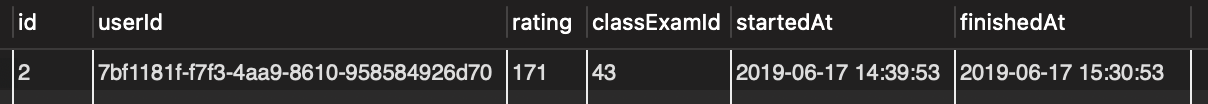
\includegraphics[width=8cm]{PrimerTabeleUser}
    \caption{Zapis za reševanje uporabnika}%TODO: figure counting
    \label{fig:example}%
\end{figure}

\iffalse
\begin{lstlisting}[language=SQL]
SELECT u.id, u.userId, u.rating, u.classExamId, a.startedAt, a.finishedAt 
FROM computed_user_ratings u JOIN exam_attempts a ON u.classExamId = a.classExamId 
WHERE u.classExamId=43;
\end{lstlisting}
\fi
\begin{figure}[h!]
    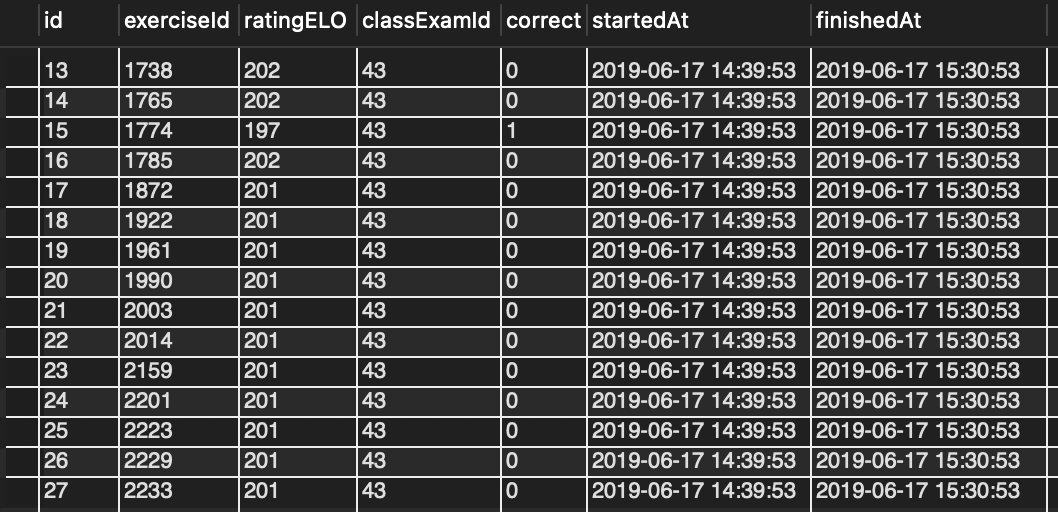
\includegraphics[width=8cm]{PrimerTabele}
    \caption{Zapisi za naloge na kvizu}%TODO: figure counting
    \label{fig:example}%
\end{figure}
\iffalse
\begin{lstlisting}[language=SQL]
SELECT e.id, e.exerciseId, e.ratingELO, e.classExamId, e.correct, a.startedAt, a.finishedAt 
FROM computed_exercise_ratings e JOIN exam_attempts a ON e.classExamId = a.classExamId 
WHERE e.classExamId=43;
\end{lstlisting}
\fi

\subsection{Trenutni rating sistem - Elo}
\label{sec:elo}
Pri oddaji kviza so pridobljeni prejšnji rating posameznih nalog v kvizu in prejšnji rating uporabnika. Za naloge in uporabnika so potem zaporedoma po nalogah izračunani novi ratingi po naslednjih enačbah:
\begin{equation}
    \mathrm{R'}_\mathrm{A}=\mathrm{R}_\mathrm{A}+\mathrm{K}\cdot \left ( \mathrm{S}_\mathrm{A}-\mathrm{E}_\mathrm{A} \right )
\end{equation}
\begin{equation}
    \mathrm{E}_\mathrm{A}=\frac{\mathrm{Q}_\mathrm{A}}{\mathrm{Q}_\mathrm{A}+\mathrm{Q}_\mathrm{B}}
\end{equation}
Kjer so
\begin{equation}
    \mathrm{Q}_\mathrm{A}=10^{\mathrm{R}_\mathrm{A}/66}\;\;\;\mathrm{Q}_\mathrm{B}=10^{\mathrm{R}_\mathrm{B}/66}
\end{equation}
$\mathrm{S}_{A}$ predstavlja dejanski izid, v primeru eQuiza 0 ali 1, $\mathrm{E}_{A}$ pa pričakovan izid.
\hfill
\\
\\
$\mathrm{K}$ je po navadi izračunan glede na statistično analizo reševanja, na različne načine~\cite{wiki},
v trenutni implementaciji ratinga pa je privzet kot konstanten z vrednostjo $4,5$.
\hfill
\\
\\
Po takem postopku je bil po zgoraj opisanih algoritmih izračunan Elo rating na filtriranih podatkih z osnovnim ratingom $200$. %\newpage
%TODO normalne?
\begin{figure}[h!]
    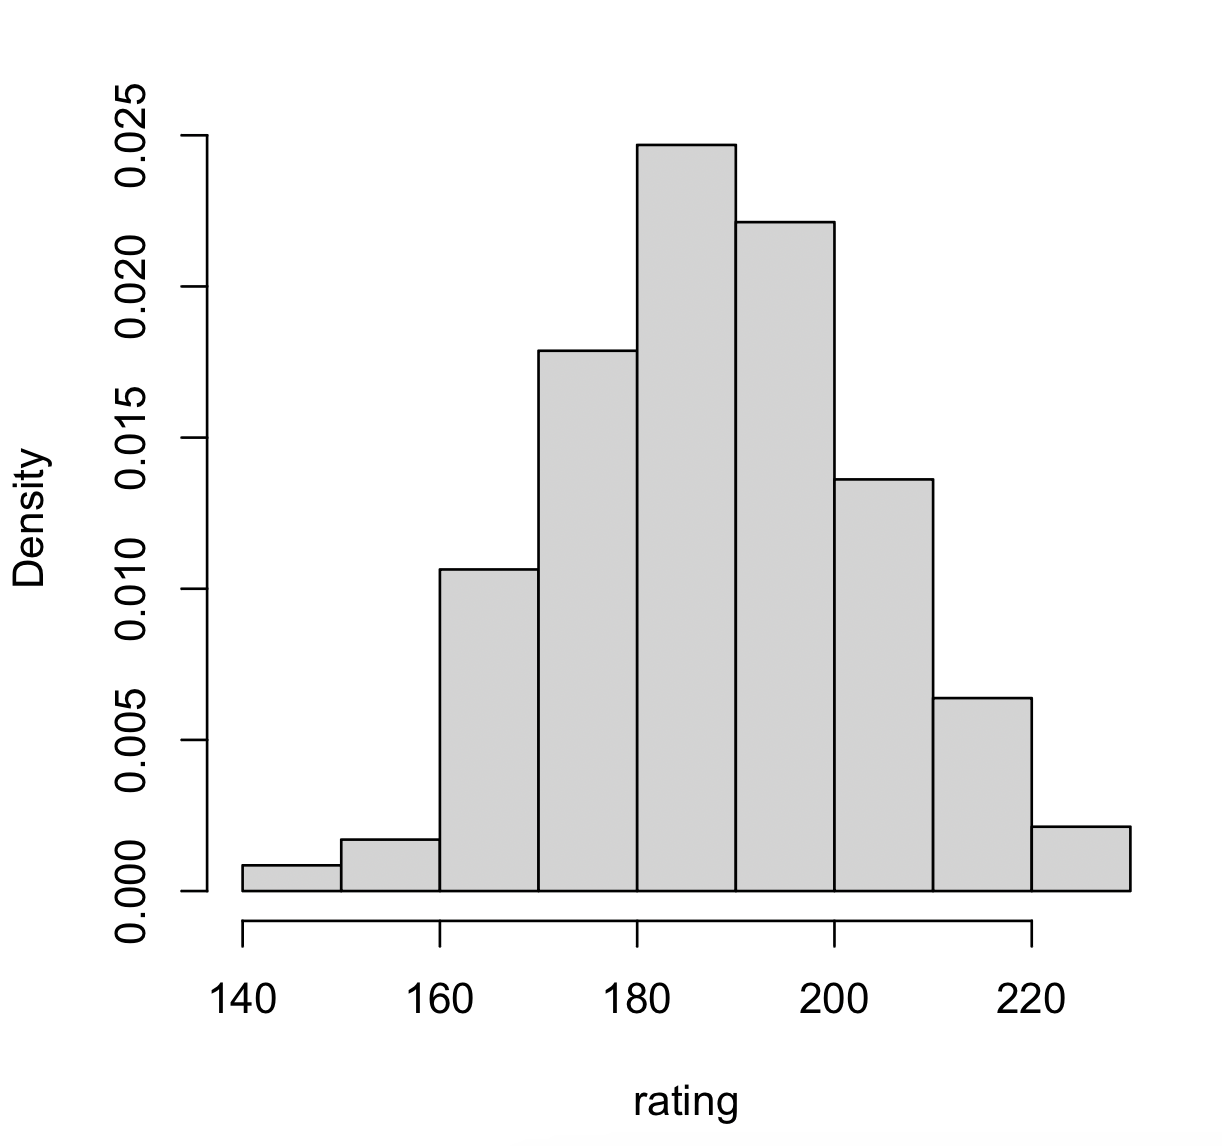
\includegraphics[width=8cm]{EloUserPrev}
    \caption{Histogram končnih Elo ratingov uporabnikov}%TODO: figure counting
    \label{fig:eloPrevU}%
\end{figure}
\begin{figure}[h!]
    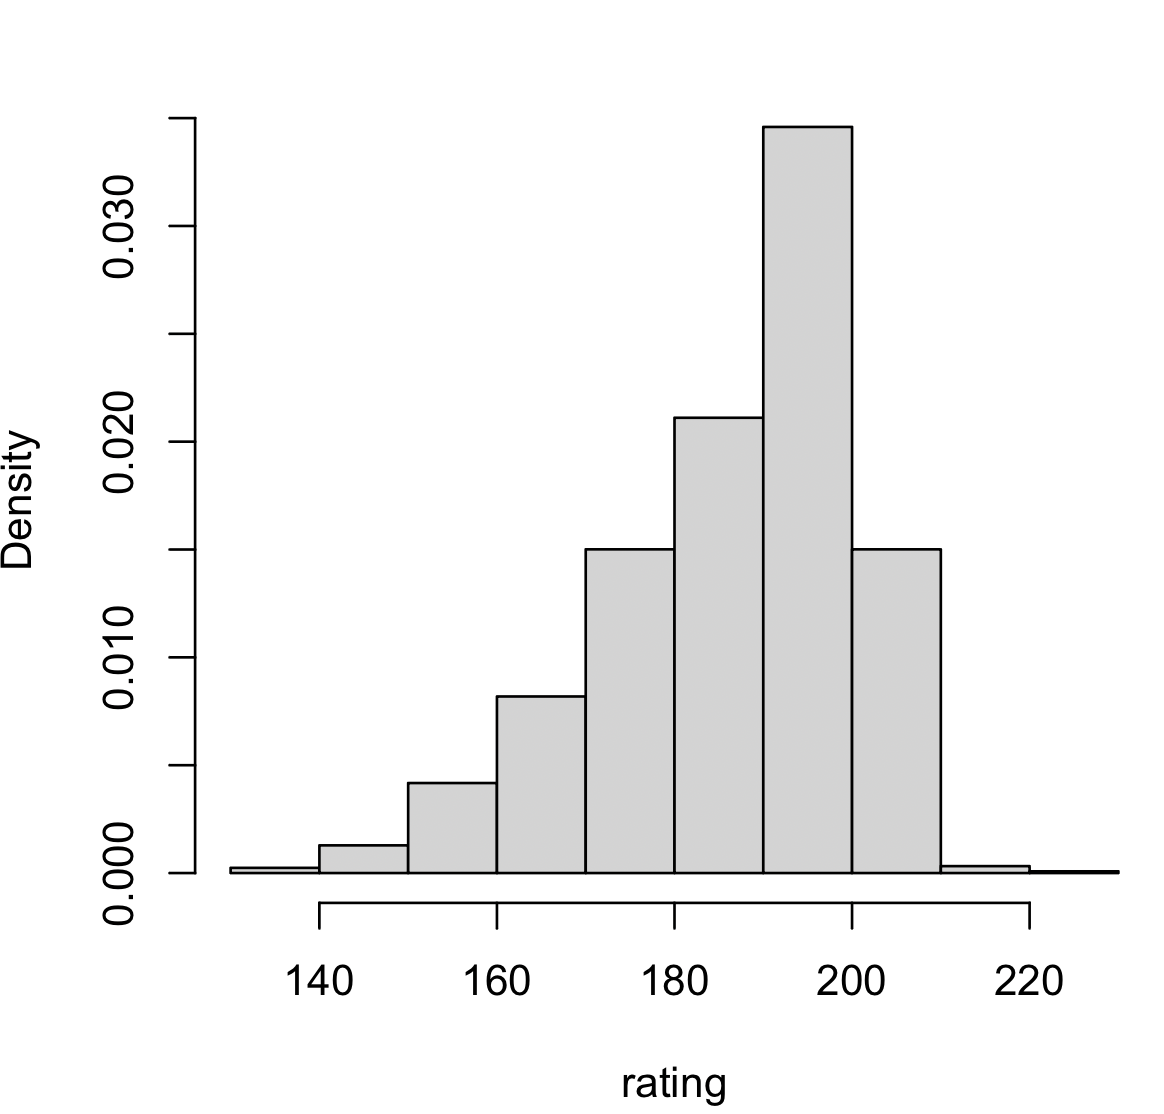
\includegraphics[width=8cm]{EloExercisePrev}
    \caption{Histogram končnih Elo ratingov nalog}%TODO: figure counting
    \label{fig:eloPrevE}%
\end{figure}
\hfill
\\
\newpage
Pri porazdelitvi ratingov uporabnikov na sliki \hyperref[fig:eloPrevU]{3}, predvsem pa nalog na sliki \hyperref[fig:eloPrevE]{4} opazimo, da so tako uporabniki, kot tudi naloge v veliki meri ocenjeni pod osnovnim ratingom $200$. Pri nalogah pa je porazdelitev celo bolj podobna eksponentni
kot normalni.

\newpage
Pri uporabi Elo ratinga, kot je implementiran sedaj, se v kontekstu eQuiza pojavijo očitne težave. Za iskanje vzroka bomo primerjali del podatkov, 
izračunanih v \hyperref[sec:glicko]{poglavju 3.4}, s podatki tranutnega Elo ratinga uporabnika, kjer rating uporabnika že po prvem reševanju pade 
(\hyperref[fig:elovsglicko]{slika 5a}), pri Glicko pa pri istem reševanju naraste (\hyperref[fig:elovsglicko]{slika 5b}).

\begin{figure}%
    \subfloat[\centering ]{{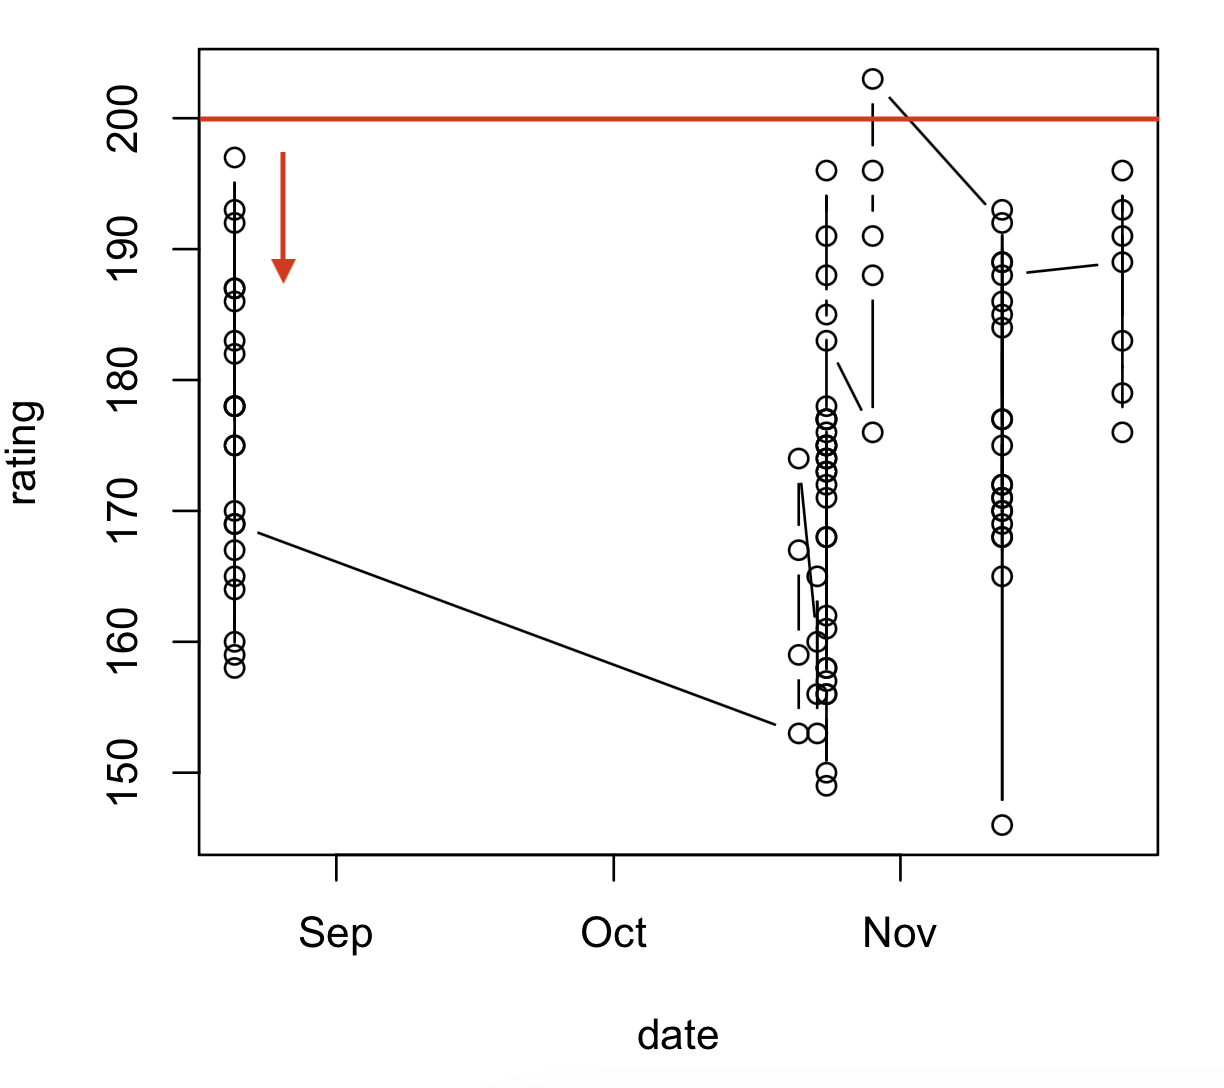
\includegraphics[width=4cm]{UserExampleElo} }}%
    \subfloat[\centering ]{{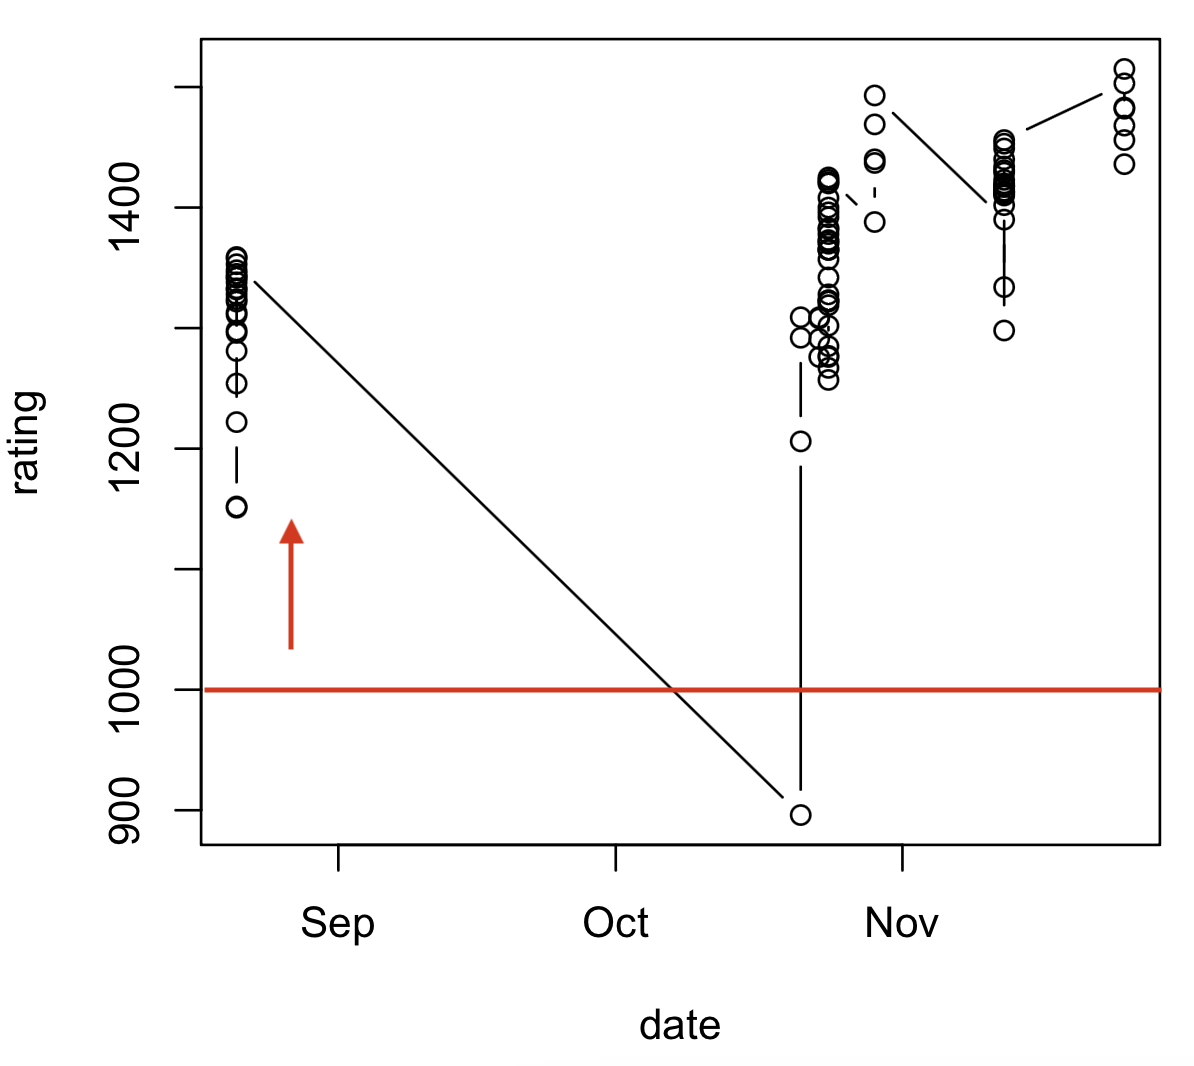
\includegraphics[width=4cm]{UserExampleGlicko} }}%
    \caption{Grafi posodobitev ratinga uporabnika za Elo (a) in Glicko (b)}%TODO: figure counting
    \label{fig:elovsglicko}%
\end{figure}

Iz tabele reševanja prvega kviza (\hyperref[fig:tabela]{slika 6}) vidimo, da je uporabnik pri pretežno pravilno rešenih nalogah (correct = 1)
dosegel negativno posodobitev ratinga pri Elo. Opazimo tudi, da je pri Elo in Glicko razlika v ratingih nalog,
kjer so pri Elo vse ocenjene pod base ratingom $200$, kar bo pri ocenjevanju pomenilo, da bodo pravilno rešene naloge
minimalno zvišale rating uporabnika, napačno rešene naloge pa ga močno znižale, saj je uporabnik napačno rešil "lahko"
nalogo. Torej uporabnik izredno težko zviša svoj rating, kar je rezultat nizko ocenjenih nalog.

\begin{figure}[h!]
    \centering
    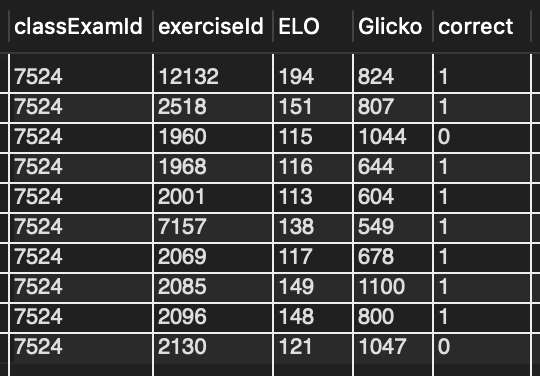
\includegraphics[width=6cm]{ExamExample}
    \caption{Tabela nalog v kvizu}%TODO: figure counting
    \label{fig:tabela}%
\end{figure}

\newpage

\begin{figure}%
    \subfloat[\centering ]{{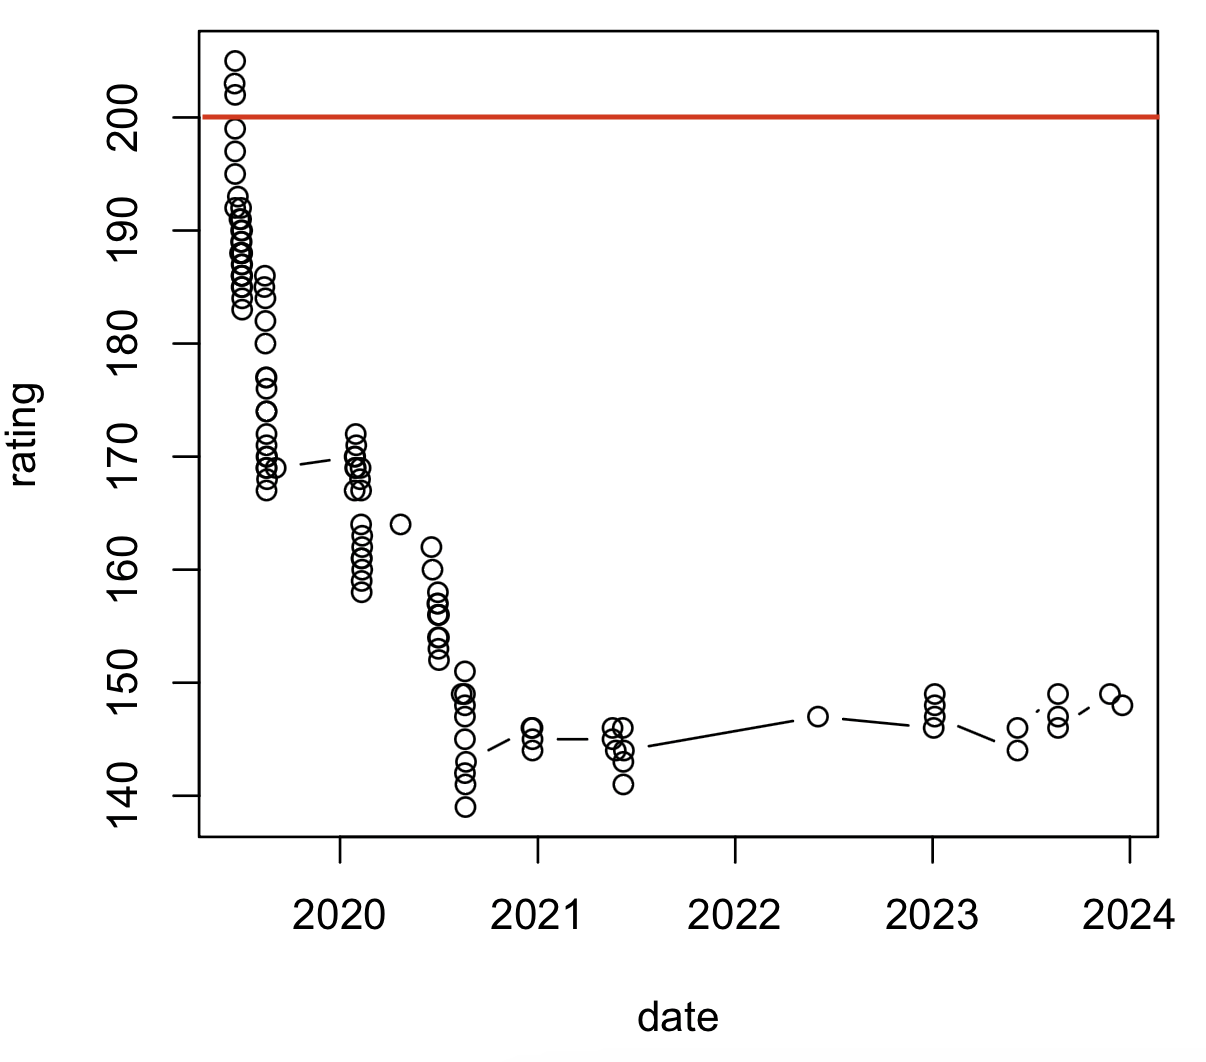
\includegraphics[width=4cm]{ExerciseExampleElo} }}%
    \subfloat[\centering ]{{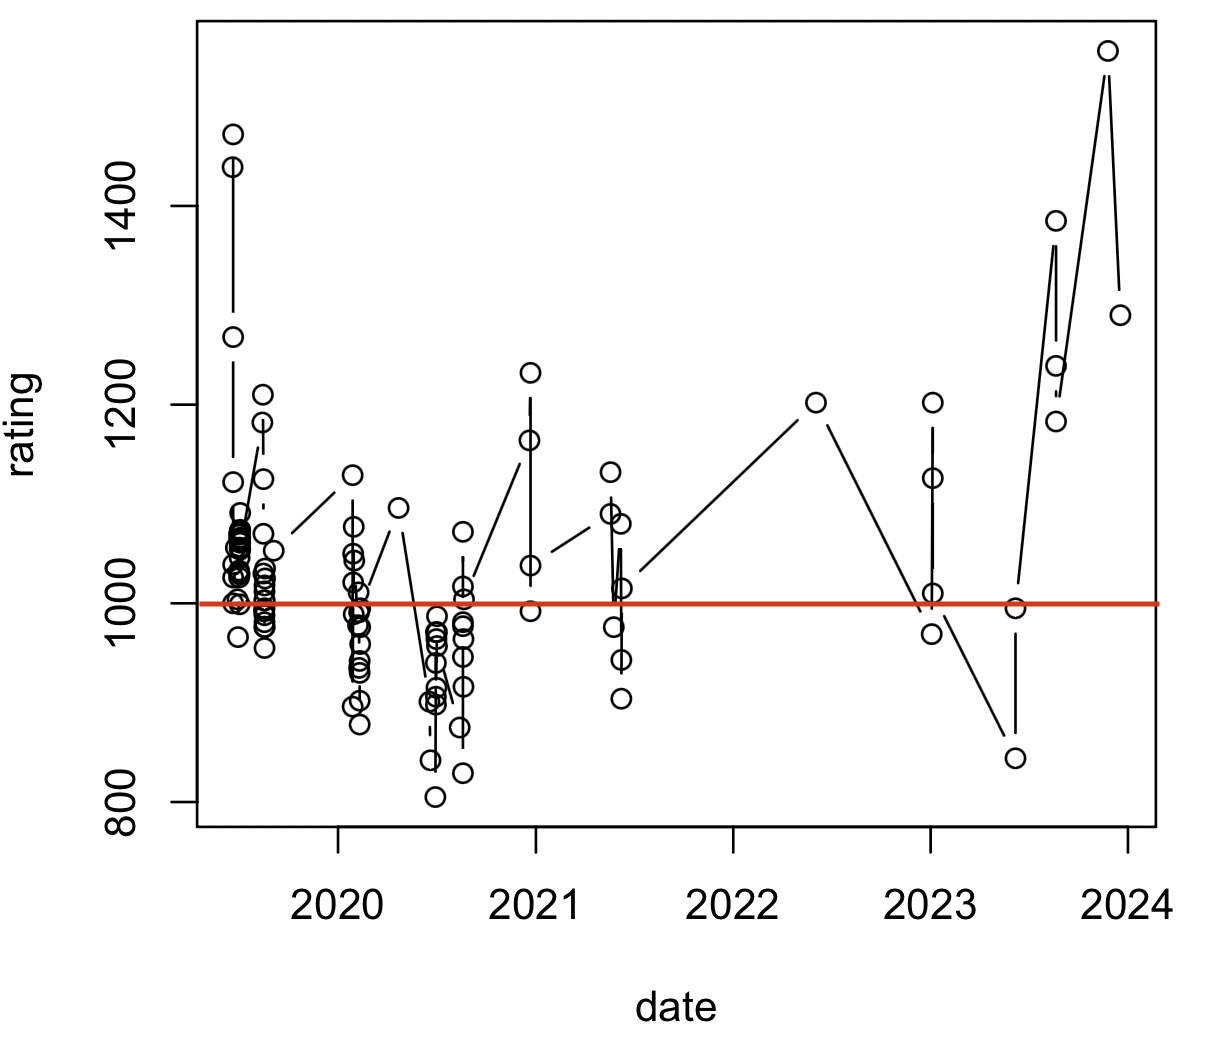
\includegraphics[width=4cm]{ExerciseExampleGlicko} }}%
    \caption{Grafi posodobitev ratinga naloge za Elo (a) in Glicko (b)}%TODO: figure counting
    \label{fig:elovsglickoe}%
\end{figure}

Pri primerjavi ratingov za nalogo (\hyperref[fig:elovsglickoe]{slika 7}), ki je pri Elo ocenjena pod osnovnim ratingom, pri Glicko pa nad, opazimo, da so pri trenutni implementaciji Elo, spremembe ratinga naloge majhne, rating pa vztrajno pada. V kolikor naloga nima možnosti
zadostno zvišati svoj rating v posamezni iteraciji pa bo pri uporabi ratinga v reševanju kvizov, pričakovano, da
bodo naloge ocenjene pod base ratingom, saj uporabniki kljub vsemu v povprečju rešijo več nalog prav kot napačno.
V podatkih pridobljenih iz eQuiza so napačno rešene naloge proti pravilno rešenim v razmerju približno 1:2.
\hfill
\\

Odzivnost ratinga na posamično nalogo, oziroma omejitev spremembe ratinga določa pri Elo ratingu parameter K (K-faktor). Nizek K-faktor predstavlja
nizko odzivnost ratinga, kar je v trenutni implementaciji očiten problem. S trenutnim K faktorjem in osnovnim ratingom se Elo izkaže za preveč togega, zato uporabniki ne uspejo pridobiti dovolj visokega ratinga, da ne bi bile vse naloge pretežno nizko ocenjene, reševanje dobrih študentov pa je torej navzgor omejeno zaradi nizkih ocen nalog. Ker ima med drugim posamezen kviz na študenta veliko večji vpliv kot na posamezno nalogo zaradi mnogih nalog v kvizu, ki tekmujejo proti študentu, bomo s pretežno nizko ocenjenimi nalogami poskrbeli, da bo študent večno nizko ocenjen. Posledično pa tudi naloge ne bodo imele, brez dovolj velikega K-faktorja možnosti, da se jim rating zviša.
\hfill
\\
\\
Kot rešitev se torej ponudi ta, da K-faktor povečamo in s tem povečamo možnost nalogam in posledično uporabnikom, da si zvišajo rating, vendar bomo
lahko s tem naredili rating nestabilen. Lahko bi uporabili spremenljiv K-faktor, za kar obstaja mnogo pristopov, najpogosteje pa se K-faktor spreminja za konstantno vrednost glede na rating razdeljen na intervale~\cite{wiki}.

\newpage
Po zvišanju trenutnega K-faktorja z $4,5$ na $32$ in premiku osnovnega ratinga na $1000$, kar je pogost nabor parametrov za Elo~\cite{wiki}, 
izgleda porazdelitev ratinga bolje (\hyperref[fig:eloU]{slika 8} in \hyperref[fig:eloU]{9}). 

\begin{figure}[h!]
    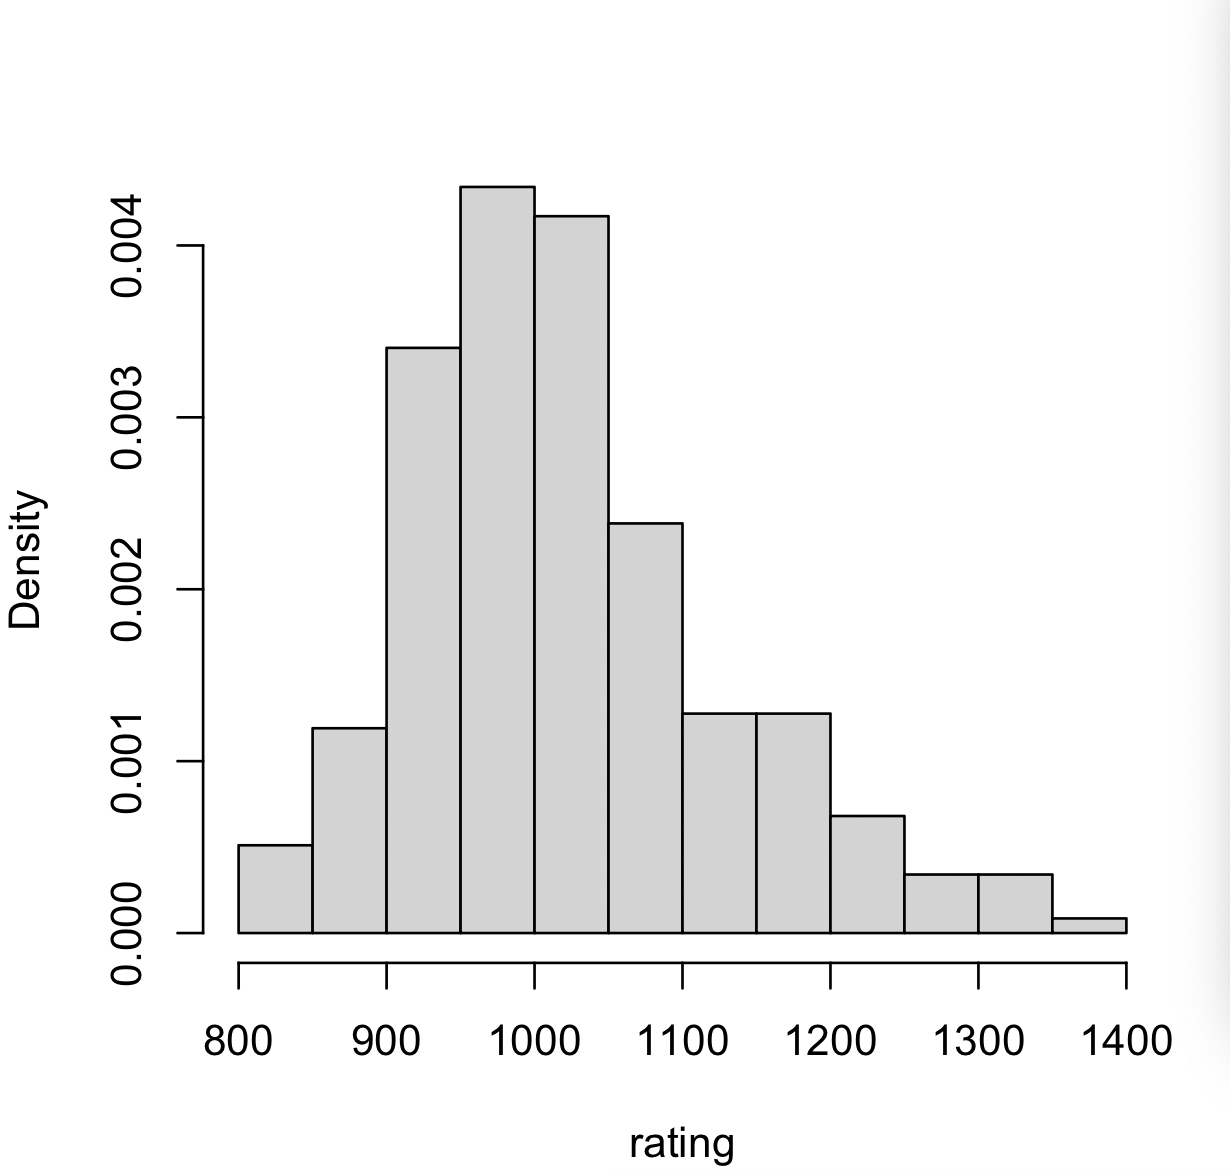
\includegraphics[width=8cm]{EloUser}
    \caption{Histogram končnih Elo ratingov nalog}%TODO: figure counting
    \label{fig:eloU}%
\end{figure}
\begin{figure}[h!]
    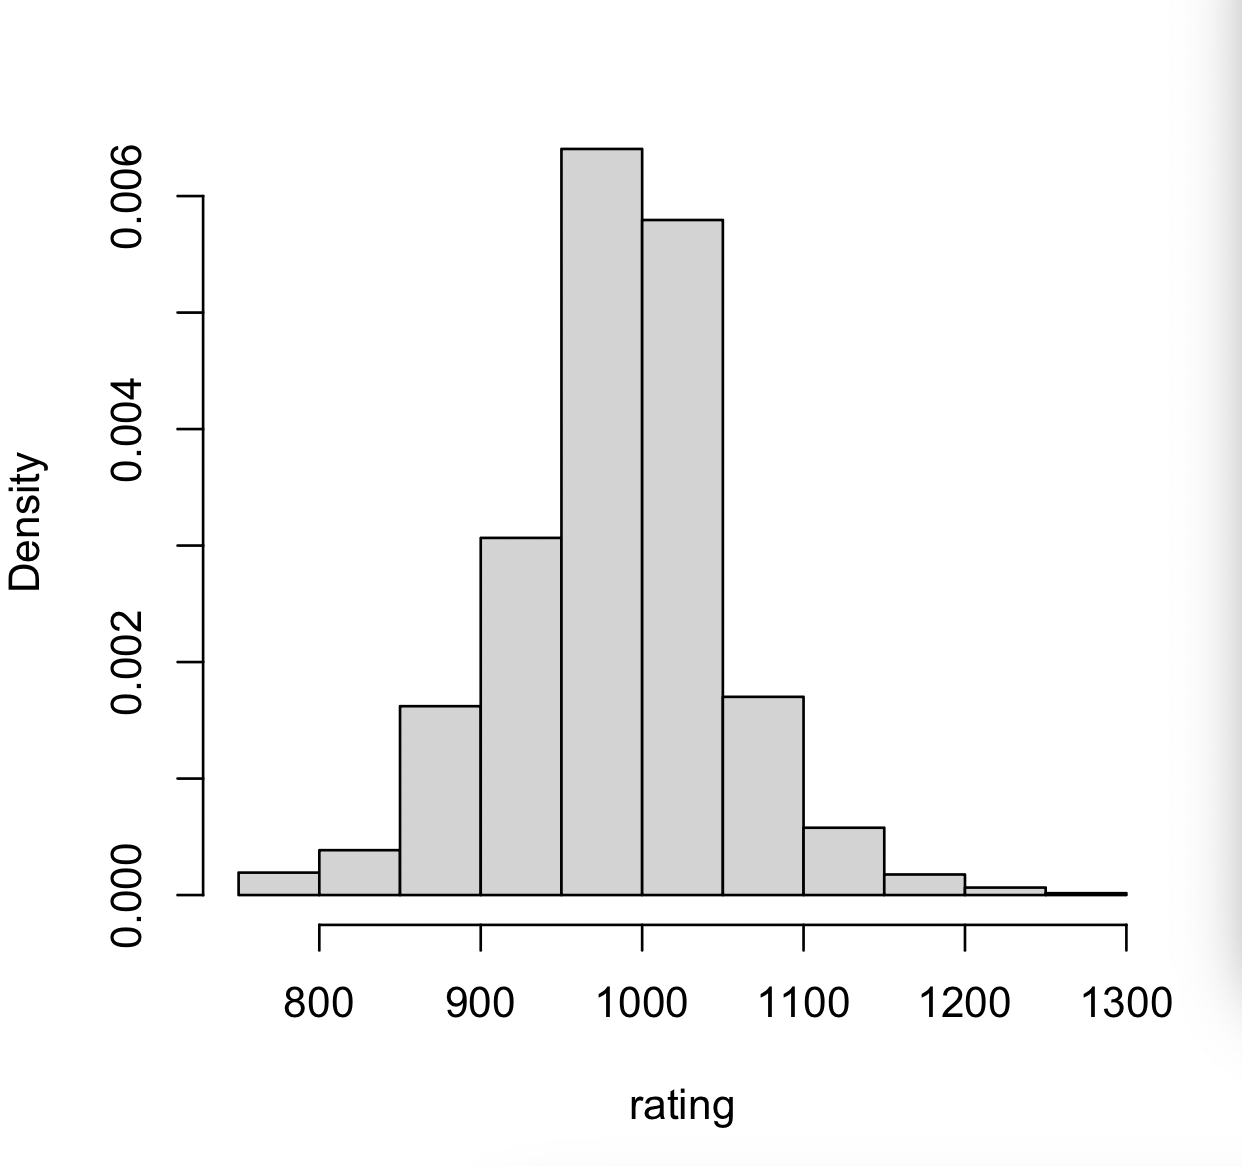
\includegraphics[width=8cm]{EloExercise}
    \caption{Histogram končnih Elo ratingov nalog}%TODO: figure counting
    \label{fig:eloE}%
\end{figure}
\newpage
Poglejmo še spremembe ratinga za konkretnega uporabnika.

\begin{figure}[h!]
    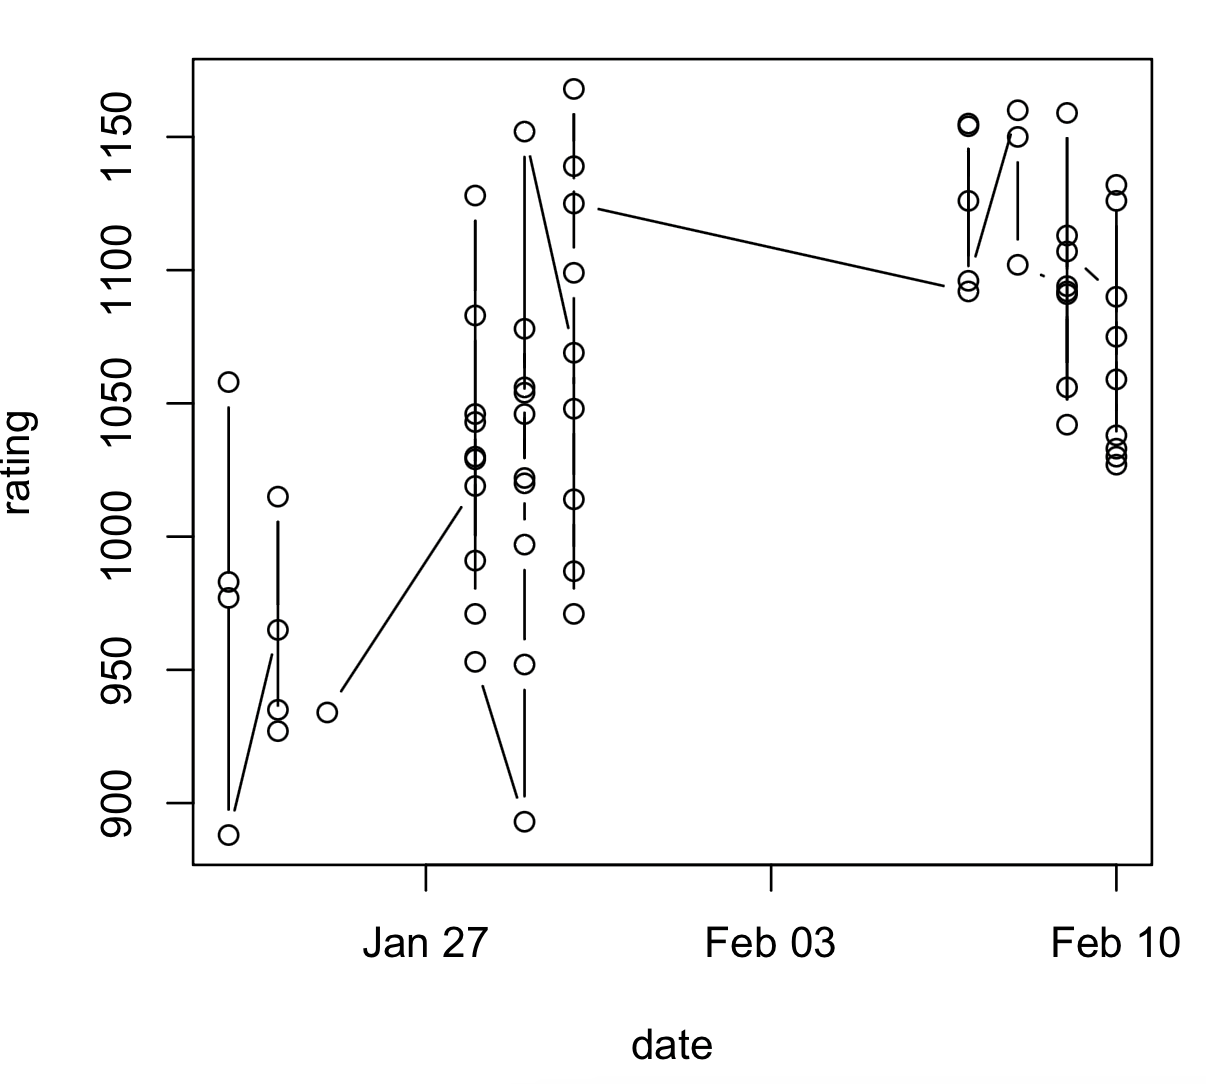
\includegraphics[width=8cm]{UserExampleSElo}
    \caption{Graf posodbitev ratinga uporabnika pri Elo}%TODO: figure counting
    \label{fig:uexse}%
\end{figure}

Na \hyperref[fig:uexse]{sliki 10} opazimo problem zvišanega K-faktorja, kar naredi Elo rating uporabnika zelo variabilen. Problem pa se da rešiti z Glicko ratingom. Glicko rating varianco v ratingu prilagaja glede na estimirano zanesljivost ratinga, kar lahko predstavlja rešitev, saj Glicko upošteva, da je rating nalog lahko razmeroma nezanesljiv, saj so ocenjevane bolj na redko kot uporabnik in tako omogoča nalogam, da se bolj razpršijo zaradi večjih prilagotiev ratinga glede na igralca, dokler njihov rating ne postane bolj zanesljiv zaradi kasnejših ocenjevanj. Če je naloga ocenjevana bolj pogosto, bo z manjšanjem deviacije prišla do natančnejšega ratinga. 
\hfill
\\
\\
To predstavlja tudi odgovor na vprašanje o zanesljivosti ratinga, če vemo, da so uporabniki kviz reševali različno mnogokrat v različno dolgih intervalih
in tako njihov rating lahko različno zanesljivo odraža pravo sposobnost reševanja uporabnikov ali težavnost nalog. V nadaljevanju je predstavljen
izračun Glicko ratinga za enake podatke.

\hfill
\\
\iffalse
\begin{figure}%
    \subfloat[\centering ]{{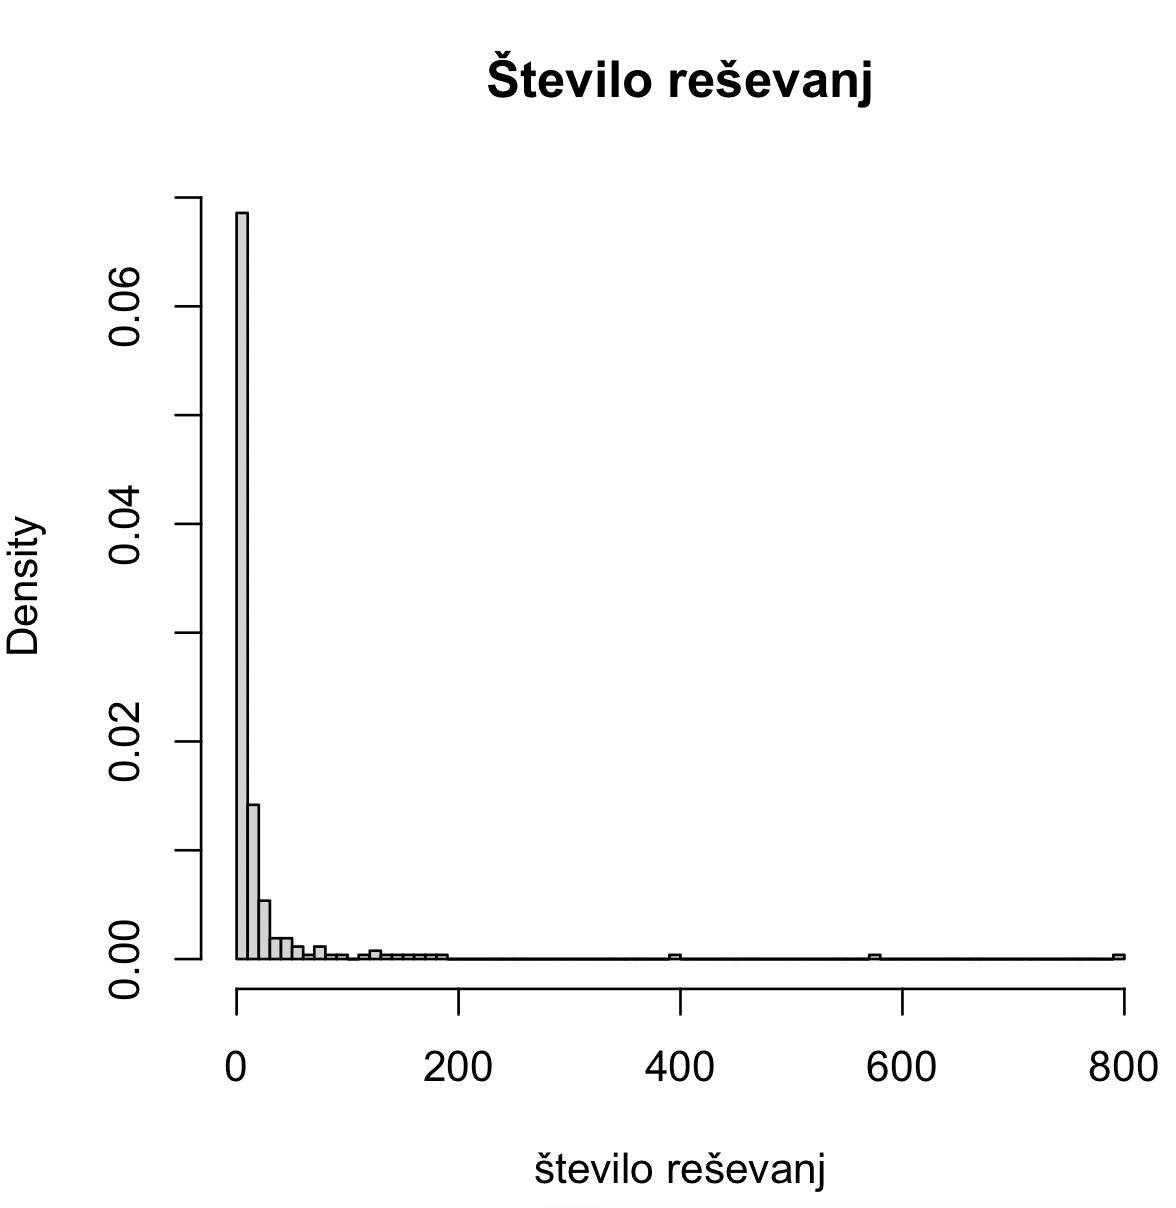
\includegraphics[width=4cm]{Resevanje} }}%
    \subfloat[\centering ]{{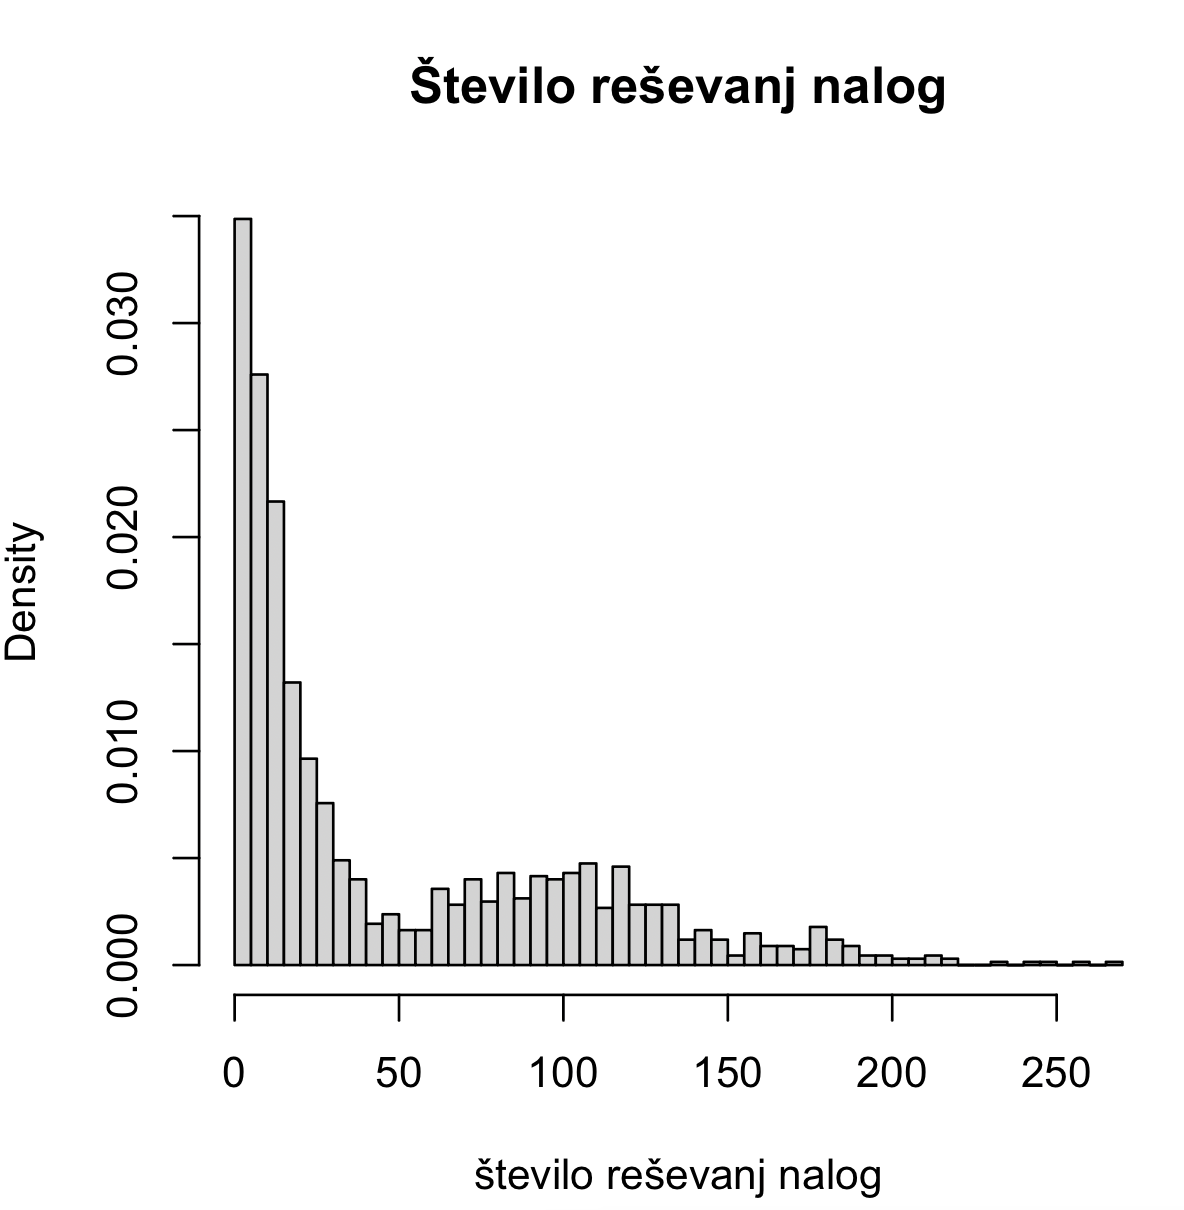
\includegraphics[width=4cm]{ResevanjeNalog} }}%
    \caption{Histogrami števila ratingov uporabnikov in nalog}%TODO: figure counting
    \label{fig:example}%
\end{figure}
\fi
%TODO: raje rate reševanja

\newpage
\subsection{Glicko rating na pridobljenih podatkih}
\label{sec:glicko}

Po enakem postopku kot Elo rating je bil zaporedno izračunan Glicko rating. Kot opisano v dokumentaciji Glicko ratinga~\cite{glickoDoc}, pa so bile naloge,
ki spadajo v isto iteracijo ocenjevanja obravnavane vsaka posebaj, kot več iger proti enako ocenjenem igralcu (uporabniku) in ne zaporedno z vmesnimi posodobitvami ratingov, kot v trenutnem rating sistemu. Osnovni rating je bil nastavljen na $1000$;
\hfill
\\
\\
Za upoštevanje časov reševanj nalog, je potreben še izračun konstante $c$ kot parameter Glicko ratinga. Kot opisano v dokumentaciji~\cite{glickoDoc} lahko $c$
izračunamo glede na to, po kolikšnem času želimo, da $\mathrm{RD}$ igralca pade na maksimalno vrednost, v tem primeru $350$. Torej če v kontekstu ocenjevanj študentov privzamemo, da bo po preteklem času enega semestra, četudi ima študent na začetku minimalen $\mathrm{RD}$, postal njegov rating nezanesljiv in pade njegov $\mathrm{RD}$ na $350$. Za tak čas je bilo vzetih $120$ dni, da pade $\mathrm{RD}$ iz povprečne vrednosti $50$ na $350$. 

\begin{equation}
    350=\sqrt{50^{2}+120\cdot c^{2}}
\end{equation}
\begin{equation}
    c\approx 32
\end{equation}


Za obdobje ocenjevanja (rating period) je bil
vzet 1 dan, kar pomeni, da se ocenjevanjem znotraj istega dne ne bo deviacija zviševala zaradi neaktivnosti. Tako obdobje lahko nastavimo poljubno,
dokumentacija Glicko ratinga~\cite{glickoDoc} pa priporoča, da povprečno na rating obdobje pride okrog 5-10 ocenjevanj, zato da je rating v posameznem obdobju dovolj natančen, hkrati pa so reševanja razdeljena v dovolj obdobij, da lahko upoštevamo obdobja, ko bi uporabnik lahko reševal, pa ni. V našem primeru bo
posamično ocenjevalno obdobje, kjer je uporabnik reševal, vedno dovolj natančno, saj se uporabnik ne more soočiti z manj kot minimalnim številom nalog na kviz in se bo tako uporabnik vedno v kvizu pomeril proti vsaj 5 nalogam. Reševanje torej ni enakomerno razporejeno ampak poteka v skupinah (posamezni
kvizi).
\newpage
Na slikah \hyperref[fig:glickoU]{11}, \hyperref[fig:glickoE]{12}, \hyperref[fig:userRD]{13} in \hyperref[fig:exerciseRD]{14} so histogrami izračunov končnih 
ratingov in deviacij uporabnikov in nalog po Glicko rating sistemu.

\begin{figure}[h!]
    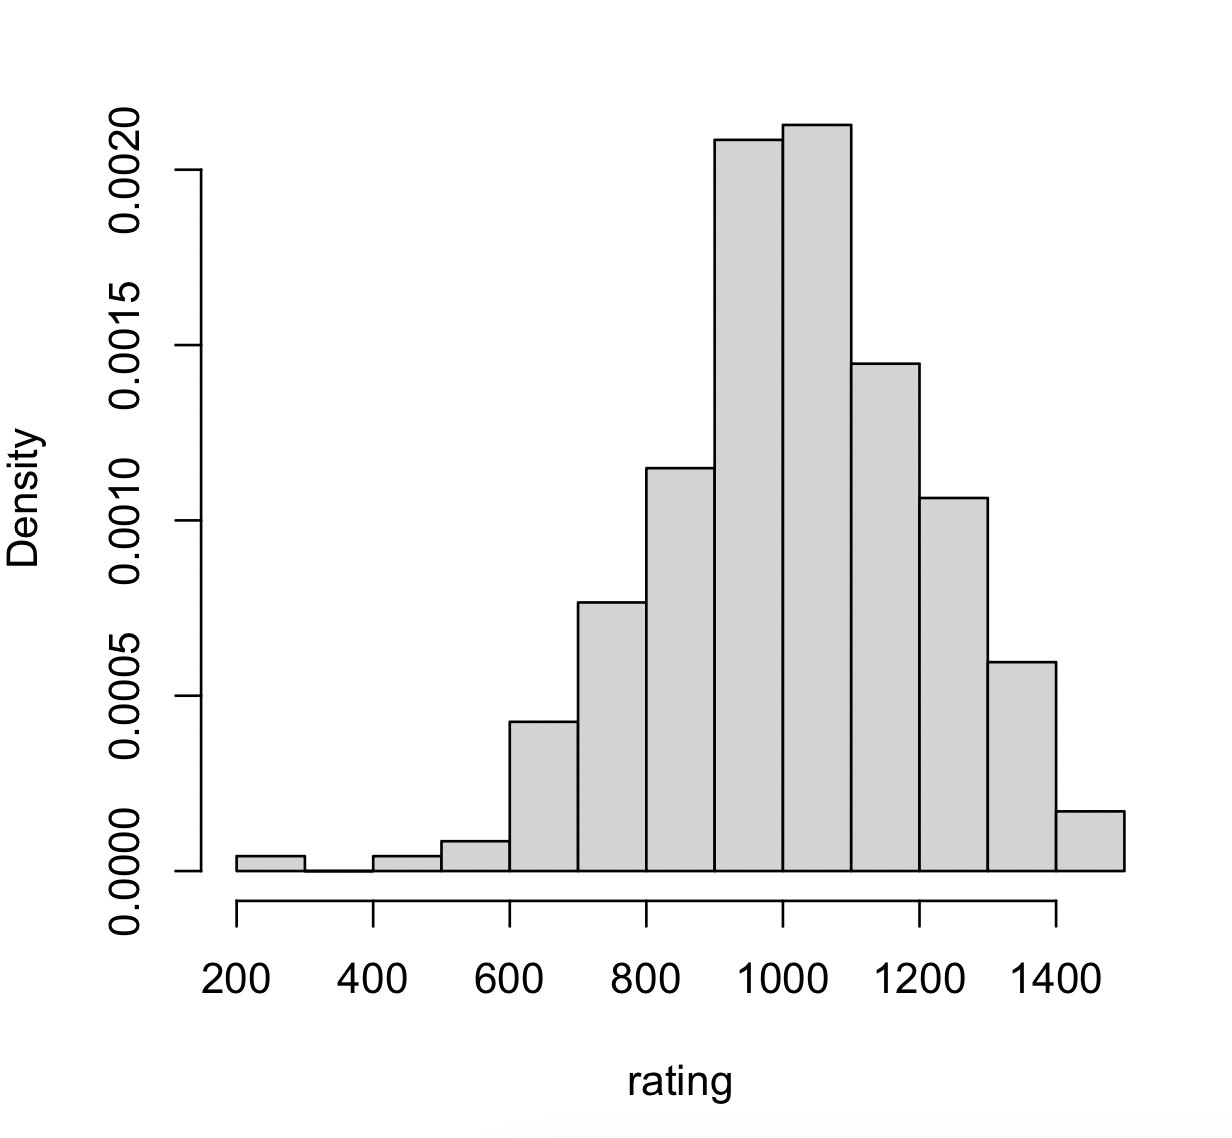
\includegraphics[width=8cm]{GlickoUser}
    \caption{Histogram končnih Glicko ratingov uporabnikov}%TODO: figure counting
    \label{fig:glickoU}%
\end{figure}
\begin{figure}[h!]
    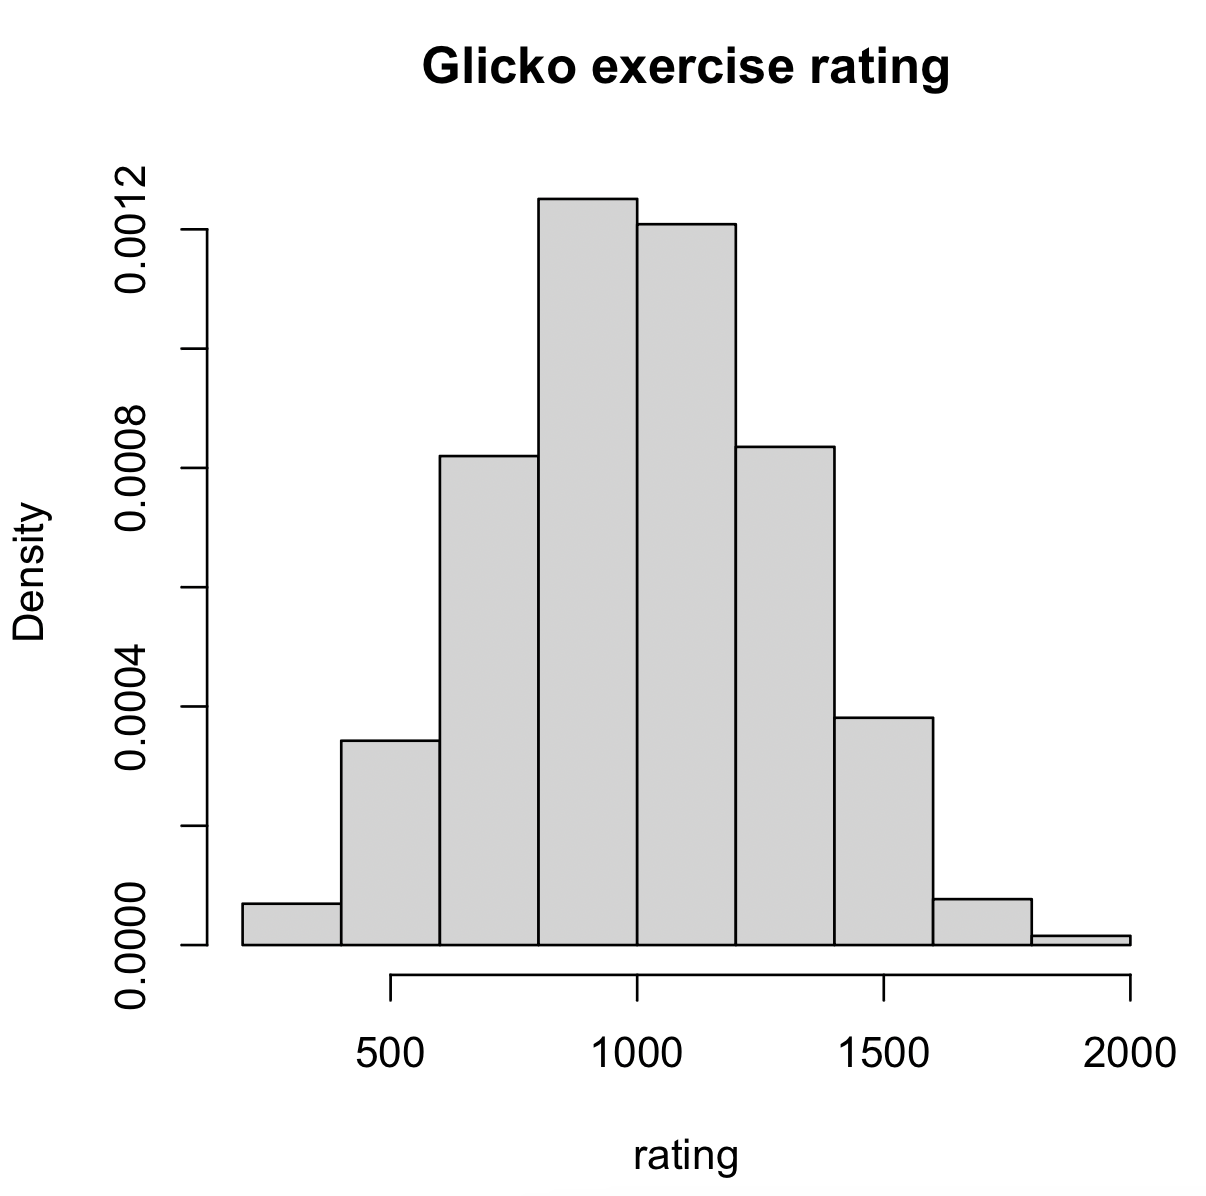
\includegraphics[width=8cm]{GlickoExercise}
    \caption{Histogram končnih Glicko ratingov nalog}%TODO: figure counting
    \label{fig:glickoE}%
\end{figure}
\begin{figure}[h!]
    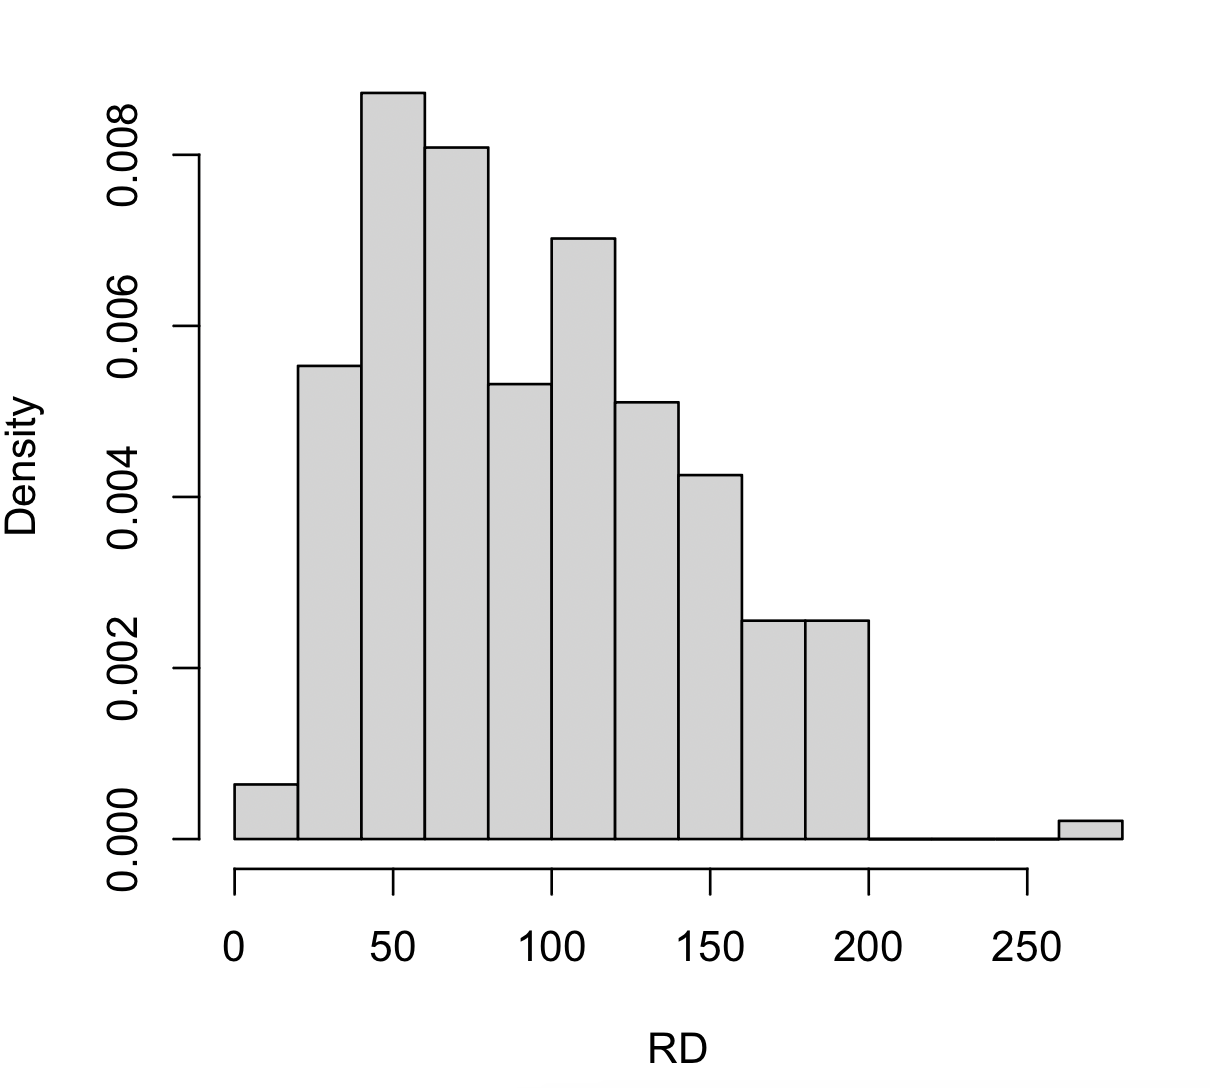
\includegraphics[width=8cm]{GlickoUserRD}
    \caption{Histogram končnih rating deviacij uporabnikov}%TODO: figure counting
    \label{fig:userRD}%
\end{figure}
\begin{figure}[h!]
    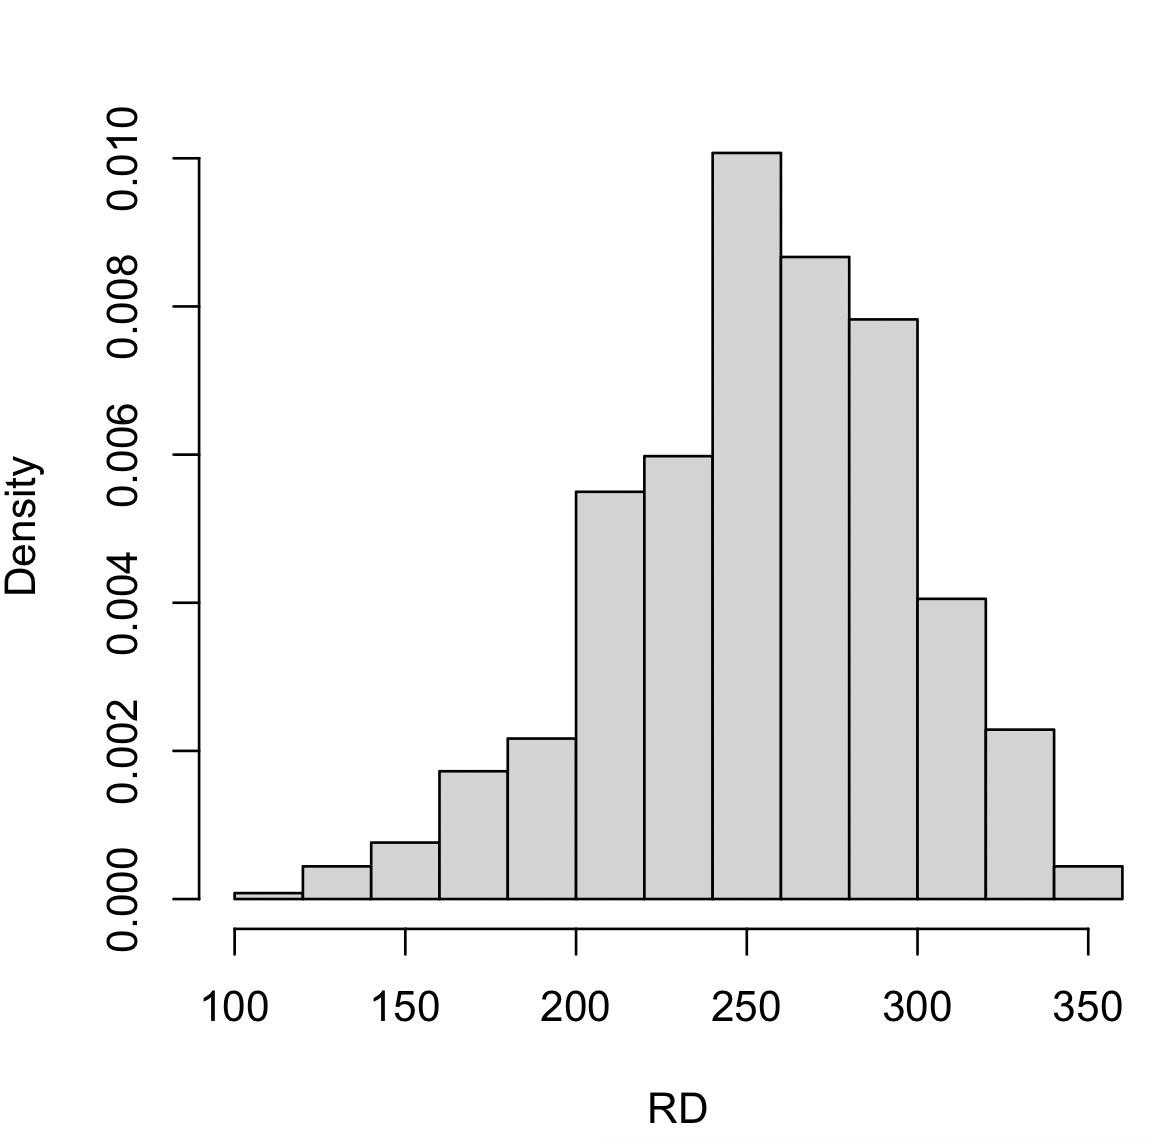
\includegraphics[width=8cm]{GlickoExerciseRD}
    \caption{Histogram končnih rating deviacij nalog}%TODO: figure counting
    \label{fig:exerciseRD}%
\end{figure}



\newpage
Opazimo, da je pri ratingu nalog $\mathrm{RD}$ povprečno večji (\hyperref[fig:exerciseRD]{slika 14}) kot pri ratingu uporabnikov (\hyperref[fig:userRD]{slika 13}), saj so naloge povprečno ocenjene bolj na redko (ocenjevanja nalog so razpršena bolj enakomerno kot reševanja uporabnikov).
\hfill
\\

Ker smo za enoto vzeli dneve moramo za razlike v datumih ocenjevanj upoštevati razliko v dnevih, kjer naj bi se njegov $\mathrm{RD}$ stalno spreminjal. Dovolj pa je, da $\mathrm{RD}$ posodobimo samo pred novim ocenjevanjem ali pa ob vpogledu v rating uporabnika, tako da upoštevamo čas od njegovega zadnjega zabeleženega ocenjevanja. Za prikaz statistike glicko ratinga v tem primeru končni izračun deviacije ni bil izveden, saj so bila ocenjevanja izvedena v zelo različnih obdobjih od 2019 do 2023 in bi tako velik del študenov imel maksimalen $\mathrm{RD}$. Za njihove ratinge to nima vpliva, saj se je med njihovimi ocenjevanji $\mathrm{RD}$ prilagajal tudi po času. Tako lahko za posameznega študenta izračunamo tudi današnji $\mathrm{RD}$ po formuli za $\mathrm{RD}$ 
po preteklem času (\hyperref[eq:rdupdate]{8}). 

\hfill
\\
Zdaj poglejmo kako se rating istega uporabnika kot v primeru pri Elo (\hyperref[fig:uexse]{sliki 10}), posodablja pri Glicko. 
Kjer so ratingi razporejeni čez razmeroma kratko obdobje, pričakujemo, da bo rating temu primerno zanesljiv in bo tako rating postopoma konvergiral, 
oziroma se bo interval zaupanja za rating zmanjšal (\hyperref[fig:uexsg]{slika 15} in \hyperref[fig:uexsgrd]{16}). 

\begin{figure}[h!]
    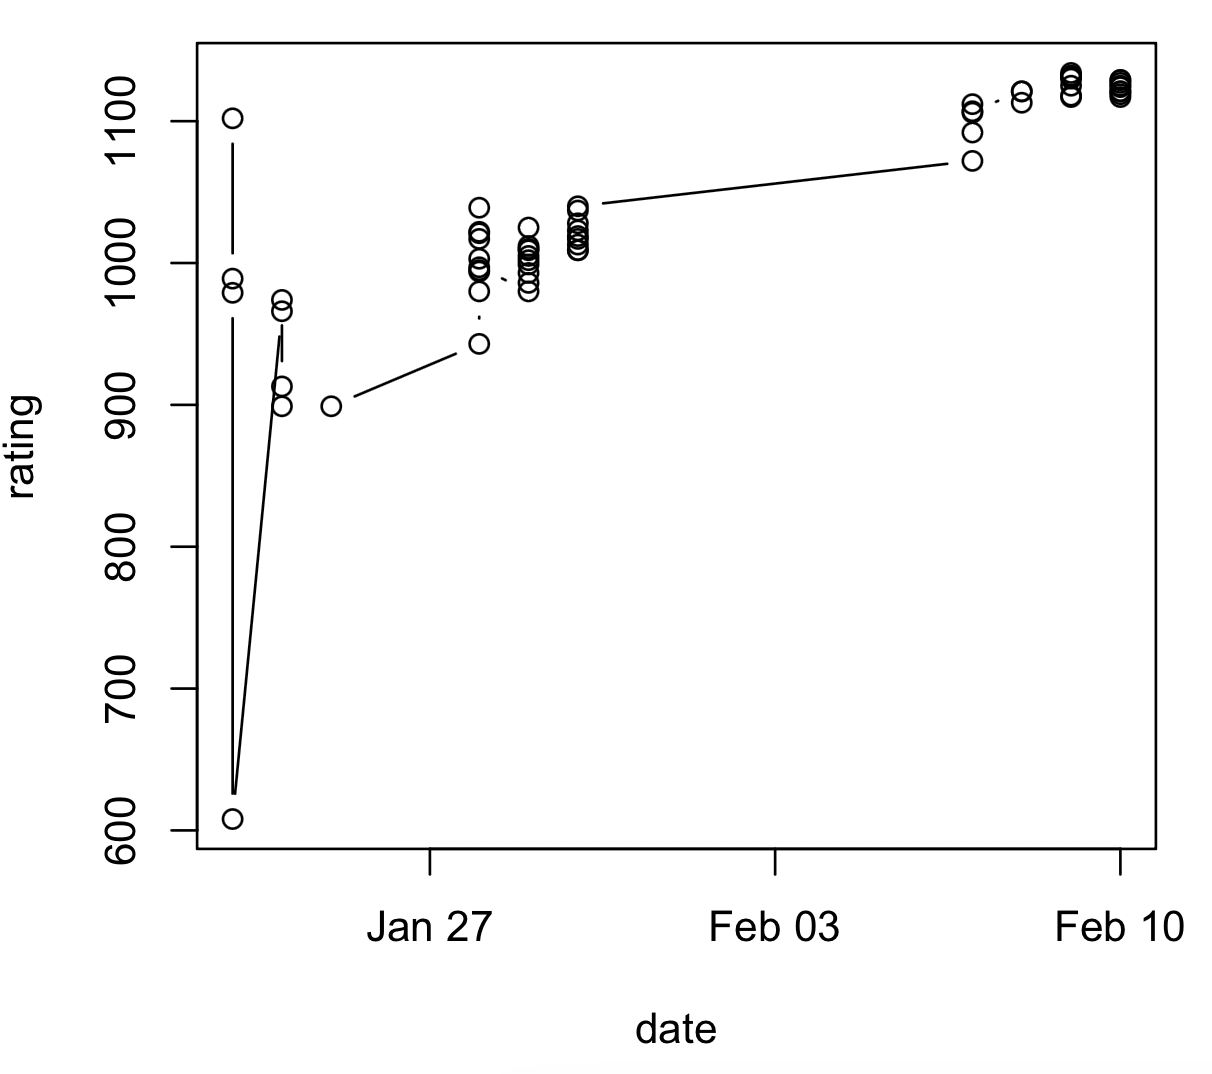
\includegraphics[width=8cm]{UserExampleSGlicko}
    \caption{Graf posodobitev ratinga za uporabnika pri Glicko}%TODO: figure counting
    \label{fig:uexsg}%
\end{figure}
\begin{figure}[h!]
    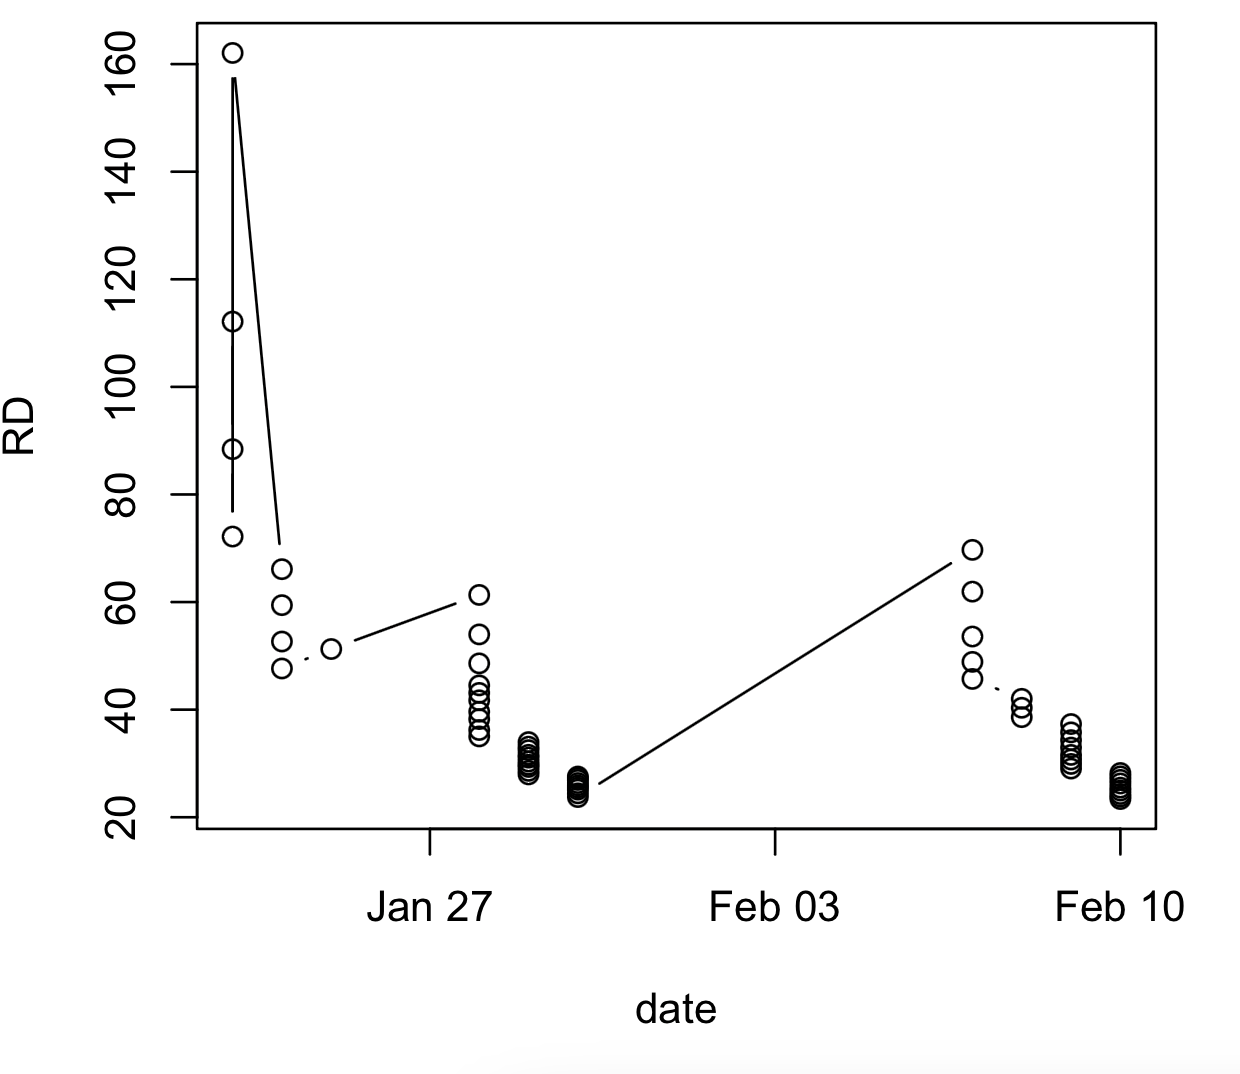
\includegraphics[width=8cm]{UserExampleSRD}
    \caption{Graf posodobitev RD za uporabnika}%TODO: figure counting
    \label{fig:uexsgrd}%
\end{figure}

\newpage
\section{Glicko za spremljanje študentov}
\label{sec:funkcionalnosti}
Z vpeljavo $\mathrm{RD}$ pridobimo v primeru študentov informacijo o sprotnem delu, saj bo $\mathrm{RD}$ manjši za študente, ki so pogosteje ocenjeni. Če bi k ratingu pripomogli tudi, na primer redni kolokviji, bi reševanje dodatnih  naključnih reševanj kvizov/nalog bilo razvidno iz manjšega $\mathrm{RD}$, kar kaže na več sprotnega dela in obratno. Predmet verjetnost in statistika, iz katerega imamo naloge na voljo tudi na eQuizu, se da na primer opraviti v celoti s sprotnimi preverjanji, kjer je snov enakomerno razdeljena na 5 kolokvijev skozi celoten semester. Torej bo študent, ki opravi samo eno preverjanje od petih ustrezno imel veliko deviacijo, saj imamo informacijo o njegovem znanju čedalje bolj nezanesljivo, ker vemo čedalje manj, koliko študent dejansko ve o statistiki, odkar je reševal tisti kolokvij.

Za nasprotnika uporabnika – nalogo, pa deviacija predstavlja kdaj je bila naloga nazadnje ocenjena, torej koliko je njena ocena zanesljiva. V primeru uporabnika, ki izbira naloge iz zbirke na eQuizu, bi lahko naloge z veliko deviacijo identificirali kot nepriljubljene (malo uporabnikov se je lotilo naloge).

%TODO tudi expected outcome

\subsection{Igrifikacija}
V kontekstu igrifikacije eQuiza, lahko ratinge, predvsem pa $\mathrm{RD}$ preslikamo v razrede iz katerih lahko bolj prijazno uporabniku spremljamo njegovo aktivnost na eQuizu. Iz statistike končnih $\mathrm{RD}$ uporabnikov lahko uporabimo kvartile in razdelimo ratinge na 4 dele:

\begin{figure}[h!]
    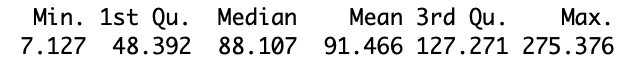
\includegraphics[width=8cm]{RDstat}
    \label{fig:example}%
\end{figure}

Tako lahko razporedimo uporabnike glede na njihove $\mathrm{RD}$:
\hfill
\\
\\
$RD\leq48,392:\;visoka\;aktivnost$
\hfill
\\
$48,392<RD\leq88,107:\;srednje\;visoka\;aktivnost$
\hfill
\\
$88,107<RD\leq127.271:\;srednje\;nizka\;aktivnost$
\hfill
\\
$127.271<RD:\;nizka\;aktivnost$
\hfill




\lstset{basicstyle=\tiny,style=SQLstyle}
\begin{lstlisting}
\end{lstlisting}
\newpage
\section{Zakjuček}
\label{sec:cnc}

Glicko rating nam doda novo informacijo glede vloženega dela uporabnika. Dobimo informacijo o količini reševanj v določenem časovnem intervalu, posledično pa tudi zanesljivost ratinga izračunanega z Glicko, kjer je zanesljivost upoštevana tudi med samim računanjem. Poleg sprotnega dela pa dobimo informacijo tudi o reševanju nalog, njihovi težavnosti in priljubljenosti. Ker pri tem poskušamo zanesljivost zvečati, lahko z vpeljavo parametriziranih nalog, ki jih tako večkrat uporabimo na preverjanjih, zvišamo zanesljivost njihovih ratingov. Če v rating vključimo še podatke iz izpitov in skupnih preverjanj, pa bo posledično rating še zanesljivejši, saj bo v isti iteraciji nalogo reševalo veliko učencev.

\hfill
\\
Kot je do sedaj algoritem operiral na trenutni podatkovni bazi eQuiza, lahko podoben algoritem uporabimo v nadaljevanju, za beleženje ratingov na enak način, kot je implementiran trenutno. Implementacija Glicko ratinga za eQuiz je na voljo skupaj z vsemi programi uporabljenimi pri navedenih izračunih na repozitoriju \href{https://github.com/MAZI2/Glicko_eQuiz}{Glicko eQuiz}. 

\hfill
\\
Za Glicko rating pa obstaja tudi bolj kompleksna izboljšana različica \href{http://www.glicko.net/glicko/glicko2.pdf}{Glicko-2}, ki upošteva tudi konsistentnost reševanja in bi s tem lahko odpravila določene nepričakovane tehnične težave pri spletnem reševanju.

\bibliographystyle{babplain}
\bibliography{cite}

\end{document}
